% Options for packages loaded elsewhere
\PassOptionsToPackage{unicode}{hyperref}
\PassOptionsToPackage{hyphens}{url}
\PassOptionsToPackage{dvipsnames,svgnames,x11names}{xcolor}
%
\documentclass[
  12pt,
]{article}
\usepackage{amsmath,amssymb}
\usepackage{setspace}
\usepackage{iftex}
\ifPDFTeX
  \usepackage[T1]{fontenc}
  \usepackage[utf8]{inputenc}
  \usepackage{textcomp} % provide euro and other symbols
\else % if luatex or xetex
  \usepackage{unicode-math} % this also loads fontspec
  \defaultfontfeatures{Scale=MatchLowercase}
  \defaultfontfeatures[\rmfamily]{Ligatures=TeX,Scale=1}
\fi
\usepackage{lmodern}
\ifPDFTeX\else
  % xetex/luatex font selection
  \setmainfont[]{Georgia}
\fi
% Use upquote if available, for straight quotes in verbatim environments
\IfFileExists{upquote.sty}{\usepackage{upquote}}{}
\IfFileExists{microtype.sty}{% use microtype if available
  \usepackage[]{microtype}
  \UseMicrotypeSet[protrusion]{basicmath} % disable protrusion for tt fonts
}{}
\makeatletter
\@ifundefined{KOMAClassName}{% if non-KOMA class
  \IfFileExists{parskip.sty}{%
    \usepackage{parskip}
  }{% else
    \setlength{\parindent}{0pt}
    \setlength{\parskip}{6pt plus 2pt minus 1pt}}
}{% if KOMA class
  \KOMAoptions{parskip=half}}
\makeatother
\usepackage{xcolor}
\usepackage[margin=1.0in]{geometry}
\usepackage{graphicx}
\makeatletter
\def\maxwidth{\ifdim\Gin@nat@width>\linewidth\linewidth\else\Gin@nat@width\fi}
\def\maxheight{\ifdim\Gin@nat@height>\textheight\textheight\else\Gin@nat@height\fi}
\makeatother
% Scale images if necessary, so that they will not overflow the page
% margins by default, and it is still possible to overwrite the defaults
% using explicit options in \includegraphics[width, height, ...]{}
\setkeys{Gin}{width=\maxwidth,height=\maxheight,keepaspectratio}
% Set default figure placement to htbp
\makeatletter
\def\fps@figure{htbp}
\makeatother
\setlength{\emergencystretch}{3em} % prevent overfull lines
\providecommand{\tightlist}{%
  \setlength{\itemsep}{0pt}\setlength{\parskip}{0pt}}
\setcounter{secnumdepth}{-\maxdimen} % remove section numbering
% definitions for citeproc citations
\NewDocumentCommand\citeproctext{}{}
\NewDocumentCommand\citeproc{mm}{%
  \begingroup\def\citeproctext{#2}\cite{#1}\endgroup}
\makeatletter
 % allow citations to break across lines
 \let\@cite@ofmt\@firstofone
 % avoid brackets around text for \cite:
 \def\@biblabel#1{}
 \def\@cite#1#2{{#1\if@tempswa , #2\fi}}
\makeatother
\newlength{\cslhangindent}
\setlength{\cslhangindent}{1.5em}
\newlength{\csllabelwidth}
\setlength{\csllabelwidth}{3em}
\newenvironment{CSLReferences}[2] % #1 hanging-indent, #2 entry-spacing
 {\begin{list}{}{%
  \setlength{\itemindent}{0pt}
  \setlength{\leftmargin}{0pt}
  \setlength{\parsep}{0pt}
  % turn on hanging indent if param 1 is 1
  \ifodd #1
   \setlength{\leftmargin}{\cslhangindent}
   \setlength{\itemindent}{-1\cslhangindent}
  \fi
  % set entry spacing
  \setlength{\itemsep}{#2\baselineskip}}}
 {\end{list}}
\usepackage{calc}
\newcommand{\CSLBlock}[1]{\hfill\break#1\hfill\break}
\newcommand{\CSLLeftMargin}[1]{\parbox[t]{\csllabelwidth}{\strut#1\strut}}
\newcommand{\CSLRightInline}[1]{\parbox[t]{\linewidth - \csllabelwidth}{\strut#1\strut}}
\newcommand{\CSLIndent}[1]{\hspace{\cslhangindent}#1}
\usepackage{longtable}
\usepackage{graphicx}
\usepackage{booktabs}
\usepackage{textcomp}
\usepackage{xcolor}
\usepackage{colortbl}
\usepackage{geometry}
\usepackage{subcaption}
\usepackage{lineno}
\usepackage{makecell}
\usepackage{pdflscape}
\definecolor{listcomment}{rgb}{0.0,0.5,0.0}
\definecolor{listkeyword}{rgb}{0.0,0.0,0.5}
\definecolor{listnumbers}{gray}{0.65}
\definecolor{listlightgray}{gray}{0.955}
\definecolor{listwhite}{gray}{1.0}
\ifLuaTeX
  \usepackage{selnolig}  % disable illegal ligatures
\fi
\IfFileExists{bookmark.sty}{\usepackage{bookmark}}{\usepackage{hyperref}}
\IfFileExists{xurl.sty}{\usepackage{xurl}}{} % add URL line breaks if available
\urlstyle{same}
\hypersetup{
  colorlinks=true,
  linkcolor={Maroon},
  filecolor={Maroon},
  citecolor={Blue},
  urlcolor={blue},
  pdfcreator={LaTeX via pandoc}}

\author{}
\date{\vspace{-2.5em}}

\begin{document}

\setstretch{1.5}
\linenumbers
\pagenumbering{gobble}

\setstretch{1}

\begin{centering}

$ $

\vspace{6cm}

\LARGE

{\bf Modular strategies for spatial mapping of multi-modal mouse brain data}

\vspace{1.0 cm}

\normalsize

Nicholas J. Tustison$^{1}$,
Min Chen$^{2}$,
Fae N. Kronman$^{3}$,
Jeffrey T. Duda$^{2}$,
Clare Gamlin$^{4}$,
Mia G. Tustison,
Michael Kunst$^{4}$,
Rachel Dalley$^{4}$,
Staci Sorenson$^{4}$,
Quanxin Wang$^{4}$,
Lydia Ng$^{4}$,
Yongsoo Kim$^{3}$, and
James C. Gee$^{2}$

\small

$^{1}$Department of Radiology and Medical Imaging, University of Virginia, Charlottesville, VA \\
$^{2}$Department of Radiology, University of Pennsylvania, Philadelphia, PA \\
$^{3}$Department of Neuroscience and Experimental Therapeutics, Penn State University, Hershey, PA \\
$^{4}$Allen Institute for Brain Science, Seattle, WA \\

\end{centering}

\vspace{3.5 cm}

\noindent

\rule{4cm}{0.4pt}

\scriptsize

Corresponding authors:\\

Nicholas J. Tustison, DSc\\
Department of Radiology and Medical Imaging\\
University of Virginia\\
\href{mailto:ntustison@virginia.edu}{\nolinkurl{ntustison@virginia.edu}}\\

James C. Gee, PhD\\
Department of Radiology\\
University of Pennsylvania\\
\href{mailto:gee@upenn.edu}{\nolinkurl{gee@upenn.edu}}

\normalsize

\newpage

\setstretch{1.5}

\section*{Abstract}\label{abstract}
\addcontentsline{toc}{section}{Abstract}

Large-scale efforts by the BRAIN Initiative Cell Census Network (BICCN)
are generating a comprehensive reference atlas of cell types in the
mouse brain. A key challenge in this effort is mapping diverse datasets,
acquired with varied imaging, tissue processing, and profiling methods,
into shared coordinate frameworks. Here, we present modular mapping
pipelines developed using the Advanced Normalization Tools Ecosystem
(ANTsX) to align MERFISH spatial transcriptomics and high-resolution
fMOST morphology data to the Allen Common Coordinate Framework (CCFv3),
and developmental MRI and LSFM data to the Developmental CCF (DevCCF).
Simultaneously, we introduce two novel methods: 1) a velocity
field--based approach for continuous interpolation across developmental
timepoints, and 2) a deep learning framework for automated brain
parcellation using minimally annotated and publicly available data. All
workflows are open-source and reproducible. We also provide general
guidance for selecting appropriate strategies across modalities,
enabling researchers to adapt these tools to new data.

\clearpage

\section{Introduction}\label{introduction}

Over the past decade, there have been significant advancements in
mesoscopic single-cell analysis of the mouse brain. It is now possible
to track single neurons\textsuperscript{1}, observe whole-brain
developmental changes at cellular resolution\textsuperscript{2},
associate brain regions with genetic composition\textsuperscript{3}, and
locally characterize neural connectivity\textsuperscript{4}. These
scientific achievements have been propelled by high-resolution profiling
and imaging techniques that enable submicron, multimodal, 3D
characterizations of whole mouse brains. Among these are micro-optical
sectioning tomography\textsuperscript{5,6}, tissue clearing
methods\textsuperscript{1,7}, spatial
transcriptomics\textsuperscript{8,9}, and single-cell genomic
profiling\textsuperscript{10}, each offering expanded specificity and
resolution for cell-level brain analysis.

Recent efforts by the NIH BRAIN Initiative have mobilized large-scale
international collaborations to create a comprehensive reference
database of mouse brain structure and function. The BRAIN Initiative
Cell Census Network has aggregated over 40 multimodal datasets from more
than 30 research groups\textsuperscript{11}, many of which are
registered to standardized anatomical coordinate systems to support
integrated analysis. Among the most widely used of these frameworks is
the Allen Mouse Brain Common Coordinate Framework
(CCFv3)\textsuperscript{12}. Other CCFs include modality-specific
references\textsuperscript{13--15} and developmental
atlases\textsuperscript{16,17} that track structural change across time.

\subsection{Mouse brain mapping
challenges}\label{mouse-brain-mapping-challenges}

Robust mapping of cell type data into CCFs is essential for integrative
analysis of morphology, connectivity, and molecular identity. However,
each modality poses unique challenges. For example, differences in
tissue processing, imaging protocols, and anatomical completeness often
introduce artifacts such as distortion, tearing, holes, and signal
dropout\textsuperscript{18--23}. Intensity differences and partial
representations of anatomy can further complicate alignment. Also, while
alternative strategies for mapping single-cell spatial transcriptomic
data exist (e.g., gene expression--based models such as
Tangram\textsuperscript{24}) this work focuses on image-based anatomical
alignment to common coordinate frameworks using spatially resolved
reference images. Given this diversity specialized strategies are often
needed to address the unique, modality-specific challenges.

Existing mapping solutions fall into three broad categories. The first
includes integrated processing platforms that provide users with mapped
datasets (e.g., Allen Brain Cell Atlas\textsuperscript{25}, Brain
Architecture Portal\textsuperscript{26},
OpenBrainMap\textsuperscript{27}, and Image and Multi-Morphology
Pipeline\textsuperscript{28}). These offer convenience and high-quality
curated data, but limited generalizability and customization. The second
category involves highly specialized pipelines tailored to specific
modalities such as histology\textsuperscript{29--31}, magnetic resonance
imaging (MRI)\textsuperscript{32--34}, microCT\textsuperscript{35,36},
light sheet fluorescence microscopy (LSFM)\textsuperscript{37,38},
flourescence micro-optical sectioning tomography
(fMOST)\textsuperscript{15,39}, and spatial transcriptomics, including
multiplexed error-robust fluorescence in situ hybridization
(MERFISH)\textsuperscript{40--42}. While effective, these solutions
often require extensive engineering effort to adapt to new datasets or
modalities. Finally, general-purpose toolkits such as
elastix\textsuperscript{43}, Slicer3D\textsuperscript{44}, and the
Advanced Normalization Tools Ecosystem (ANTsX)\textsuperscript{45} have
all been applied to mouse brain mapping scenarios. These toolkits
support modular workflows that can be flexibly composed from reusable
components, offering a powerful alternative to rigid, modality-specific
solutions. However, their use often requires familiarity with pipeline
modules, parameter tuning, and tool-specific conventions which can limit
adoption.

Building on this third category, we describe a set of modular,
ANTsX-based pipelines specifically tailored for mapping diverse mouse
brain data into standardized anatomical frameworks. These include two
new pipelines: a velocity field--based interpolation model that enables
continuous transformations across developmental timepoints of the
DevCCF, and a template-based deep learning pipeline for whole brain
segmentation (i.e., brain extraction) and structural anatomical regional
labeling of the brain (i.e., brain parcellation) requiring minimal
annotated data. In addition, we include two modular pipelines for
aligning MERFISH and fMOST datasets to the Allen CCFv3. While the
MERFISH dataset was previously published as part of earlier BICCN
efforts\textsuperscript{46}, the full image processing and registration
workflow had not been described in detail until now. The fMOST workflow,
by contrast, was developed internally to support high-resolution
morphology mapping and has not been previously published in any form.
Both pipelines were built using ANTsX tools, adapted for collaborative
use with the Allen Institute, and are now released as fully
reproducible, open-source workflows to support reuse and extension by
the community. To facilitate broader adoption, we also provide general
guidance for customizing these strategies across imaging modalities and
data types. We first introduce key components of the ANTsX toolkit,
which provide a basis for all of the mapping workflows described here,
and then detail the specific contributions made in each pipeline.

\subsection{The Advanced Normalization Tools Ecosystem
(ANTsX)}\label{the-advanced-normalization-tools-ecosystem-antsx}

The Advanced Normalization Tools Ecosystem (ANTsX) has been used in a
number of applications for mapping mouse brain data as part of core
processing steps in various workflows\textsuperscript{31,46--49},
particularly its pairwise, intensity-based image registration
capabilities\textsuperscript{50} and bias field
correction\textsuperscript{51}. Historically, ANTsX development is based
on foundational approaches to image mapping\textsuperscript{52--54},
especially in the human brain, with key contributions such as the
Symmetric Normalization (SyN) algorithm\textsuperscript{50}. It has been
independently evaluated in diverse imaging domains including multi-site
brain MRI\textsuperscript{55}, pulmonary CT\textsuperscript{56}, and
multi-modal brain tumor registration\textsuperscript{57}. More recent
contributions for mouse-specific applications showcase multimodal
template generation\textsuperscript{16} and anatomy-aware
registration\textsuperscript{58} ANTsX functionality.

Beyond registration, ANTsX provides functionality for template
generation\textsuperscript{59}, segmentation\textsuperscript{60},
preprocessing\textsuperscript{51,61}, and deep
learning\textsuperscript{45}. It has demonstrated strong performance in
consensus labeling\textsuperscript{62}, brain tumor
segmentation\textsuperscript{63}, and cardiac motion
estimation\textsuperscript{64}. Built on the Insight Toolkit
(ITK)\textsuperscript{65}, ANTsX benefits from open-source contributions
while supporting continued algorithm evaluation and innovation. In the
context of mouse brain data, ANTsX provides a robust platform for
developing modular pipelines to map diverse imaging modalities into
CCFs. These tools span multiple classes of mapping problems:
cross-modality image registration, landmark-driven alignment, temporal
interpolation across developmental stages, and deep learning--based
segmentation. As such, they also serve as illustrative case studies for
adapting ANTsX tools to other use cases. We describe both shared
infrastructure and targeted strategies adapted to the specific
challenges of each modality. This paper highlights usage across distinct
BICCN projects such as spatial transcriptomic data from MERFISH,
structural data from fMOST, and multimodal developmental data from LSFM
and MRI.

\subsection{Novel ANTsX-based open-source
contributions}\label{novel-antsx-based-open-source-contributions}

We introduce two novel contributions to ANTsX developed as part of
collabortive efforts in creating the Developmental Common Coordinate
Framework (DevCCF)\textsuperscript{16}. First, we present an open-source
velocity field--based interpolation framework for continuous mapping
across the sampled embryonic and postnatal stages of the DevCCF
atlas\textsuperscript{16}. This functionality enables biologically
plausible interpolation between timepoints via a time-parameterized
diffeomorphic velocity model\textsuperscript{66}, inspired by previous
work\textsuperscript{67}. Second, we present a deep learning pipeline
for structural parcellation of the mouse brain from multimodal MRI data.
This includes two novel components: 1) a template-derived brain
extraction model using augmented data from two ANTsX-derived template
datasets\textsuperscript{68,69}, and 2) a template-derived parcellation
model trained on DevCCF P56 labelings mapped from the AllenCCFv3. This
pipeline demonstrates how ANTsX tools and public resources can be
leveraged to build robust anatomical segmentation pipelines with minimal
annotated data. We independently evaluate this framework using a
longitudinal external dataset\textsuperscript{70}, demonstrating
generalizability across specimens and imaging protocols. All components
are openly available through the R and Python ANTsX packages, with
general-purpose functionality documented in a reproducible,
cross-platform tutorial (\url{https://tinyurl.com/antsxtutorial}). Code
specific to this manuscript, including scripts to reproduce the novel
contributions and all associated evaluations, is provided in a dedicated
repository (\url{https://github.com/ntustison/ANTsXMouseBrainMapping}).
Additional tools for mapping spatial transcriptomic (MERFISH) and
structural (fMOST) data to the AllenCCFv3 are separately available at
(\url{https://github.com/dontminchenit/CCFAlignmentToolkit}).

\clearpage
\newpage

\section{Results}\label{results}

\begin{figure*}
\centering
\begin{subfigure}[t]{0.49\textwidth}
\centering
\includegraphics[width=0.99\textwidth]{Figures/merfishPipeline.pdf}
\caption{}
\end{subfigure} 
\begin{subfigure}[t]{0.49\textwidth}
\centering
\includegraphics[width=0.99\textwidth]{Figures/fmostPipeline.pdf}
\caption{}
\end{subfigure}
\caption{Diagram of the two ANTsX-based pipelines for mapping (a) MERFISH
          and (b)fMOST data into the space of AllenCCFv3.  Each generates
         the requisite transforms to map individual images
         to the CCF.}
\label{fig:allenpipelines}
\end{figure*}

\subsection{AllenCCFv3 brain image
mapping}\label{allenccfv3-brain-image-mapping}

\subsubsection{Mapping multiplexed error-robust fluorescence in situ
hybridization (MERFISH)
data}\label{mapping-multiplexed-error-robust-fluorescence-in-situ-hybridization-merfish-data}

\textbf{Overview.} We developed an ANTsX-based pipeline to map spatial
transcriptomic MERFISH data into the AllenCCFv3
(Figure\,\ref{fig:allenpipelines}(a)). This approach was used in recent
efforts to create a high-resolution transcriptomic atlas of the mouse
brain\textsuperscript{46}. The pipeline maps spatial gene expression
patterns from MERFISH onto anatomical labels in the AllenCCFv3. It
includes MERFISH-specific preprocessing steps such as section
reconstruction, label generation from spatial transcriptomic maps, and
anatomical correspondence mapping. Alignment proceeds in two stages: 1)
3D affine registration and section matching of the AllenCCFv3 to the
MERFISH data, and 2) linear + deformable 2D section-wise alignment
between matched MERFISH and atlas slices. These transformations are
concatenated to produce a complete mapping from each MERFISH data to
AllenCCFv3.

\textbf{Data.} MERFISH imaging was performed on cryosectioned brains
from C57BL/6 mice using previously described
protocols\textsuperscript{46}. Brains were placed into an optimal
cutting temperature (OCT) compound (Sakura FineTek 4583) stored at
-80\(^\circ\). The fresh frozen brain was sectioned at 10 \(\mu\)m on
Leica 3050 S cryostats at intervals of 200\,\(\mu\)m to evenly cover the
brain. A set of 500 genes was selected to distinguish \(\sim5200\)
transcriptomic clusters. Raw MERSCOPE data were decoded using Vizgen
software (v231). Cell segmentation was performed using
Cellpose\textsuperscript{71,72} based on DAPI and PolyT stains which was
propagated to adjacent slices across z-planes. Each MERFISH cell was
assigned a transcriptomic identity by mapping to a scRNA-seq reference
taxonomy.

\textbf{Evaluation.} Alignment quality was evaluated iteratively by an
expert anatomist, guided by expected gene-marker correspondences to
AllenCCFv3 regions. As previously reported\textsuperscript{46}, further
assessment of the alignment showed that, of the 554 terminal regions
(gray matter only in the AllenCCFv3), only seven small subregions did
not contain cells from the MERFISH dataset post registration: frontal
pole, layer 1 (FRP1), FRP2/3, FRP5; accessory olfactory bulb, glomerular
layer (AOBgl); accessory olfactory bulb, granular layer (AOBgr);
accessory olfactory bulb, mitral layer (AOBmi); and accessory supraoptic
group (ASO). A broader discussion of evaluation design choices and
evaluation rationale is included in the Discussion.

\subsubsection{Mapping fluorescence micro-optical sectioning tomography
(fMOST)
data}\label{mapping-fluorescence-micro-optical-sectioning-tomography-fmost-data}

\textbf{Overview.} We also constructed a pipeline for mapping fMOST
images to the AllenCCFv3 using ANTsX
(Figure\,\ref{fig:allenpipelines}(b)). The approach leverages a
modality-specific average fMOST atlas as an intermediate target, adapted
from previous work in human and mouse brain
mapping\textsuperscript{12,15,16,59,73--76}. The atlas was constructed
from 30 fMOST images selected to capture representative variability in
anatomical shape and image intensity across the population.
Preprocessing includes cubic B-spline downsampling to match the
25\,\(\mu\)m isotropic AllenCCFv3 resolution, stripe artifact
suppression using a 3D notch filter implemented with SciPy's
frequency-domain filtering tools, and N4 bias field
correction\textsuperscript{51}. A one-time, annotation-driven alignment
registers the fMOST atlas to AllenCCFv3 using landmark-based
registration of key structures. This canonical mapping is then reused.
New fMOST specimens are first aligned to the fMOST atlas using standard
intensity-based registration, and the concatenated transforms yield full
spatial normalization to the AllenCCFv3. This same mapping can be
applied to neuron reconstructions to facilitate population-level
analysis of morphology and spatial distribution.

\textbf{Data.} fMOST imaging was performed on 55 mouse brains with
sparse transgenic labeling of neuron populations\textsuperscript{77,78}
using the high-throughput fMOST platform\textsuperscript{79,80}. Voxel
resolution was \(0.35\times 0.35\times 1.0\) \(\mu\)m\(^3\). Two imaging
channels were acquired: GFP-labeled neuron morphology (green), and
propidium iodide counterstaining for cytoarchitecture (red). Alignment
was performed using the red channel for its greater contrast, though
multi-channel mapping is also supported.

\textbf{Evaluation.} The canonical mapping from the fMOST atlas to
AllenCCFv3 was evaluated using both quantitative and qualitative
approaches. Dice similarity coefficients were computed between
corresponding anatomical labels in the fMOST atlas and AllenCCFv3
following registration. These labels were manually annotated or adapted
from existing atlas segmentations. Representative Dice scores included:
whole brain (0.99), caudate putamen (0.97), fimbria (0.91), posterior
choroid plexus (0.93), anterior choroid plexus (0.96), optic chiasm
(0.77), and habenular commissure (0.63). In addition to these
quantitative assessments, each registered fMOST specimen was evaluated
qualitatively. An expert anatomist reviewed alignment accuracy and
confirmed structural correspondence. Neuron reconstructions from
individual brains were also transformed into AllenCCFv3 space, and their
trajectories were visually inspected to confirm anatomical plausibility
and preservation of known projection patterns. A broader discussion of
evaluation design choices and evaluation rationale is included in the
Discussion.

\subsection{Continuously mapping the DevCCF developmental
trajectory}\label{continuously-mapping-the-devccf-developmental-trajectory}

\begin{figure}
\centering
\includegraphics[width=0.99\textwidth]{Figures/lowerLeftPanel.pdf} \caption{The
spatial transformation between any two time points within the continuous DevCCF
longitudinal developmental trajectory is available through the use of ANTsX
functionality for generating a velocity flow model.}
\label{fig:devccfvelocity}
\end{figure}

The DevCCF is an openly accessible resource for the mouse brain research
community\textsuperscript{16}, comprising symmetric, multi-modal MRI and
LSFM templates generated using the ANTsX framework\textsuperscript{59}.
It spans key stages of mouse brain development (E11.5, E13.5, E15.5,
E18.5, P4, P14, and P56) and includes structural labels defined by a
developmental ontology. The DevCCF was constructed in coordination with
the AllenCCFv3 to facilitate integration across atlases and data types.

Although this collection provides broad developmental coverage, its
discrete sampling limits the ability to model continuous transformations
across time. To address this, we developed a velocity flow--based
modeling approach that enables anatomically plausible, diffeomorphic
transformations between any two continuous time points within the DevCCF
range. Unlike traditional pairwise interpolation, which requires
sequential warping through each intermediate stage, this model, defined
by a time-varying velocity field (i.e., a smooth vector field defined
over space and time that governs the continuous deformation of an image
domain), allows direct computation of deformations between any two time
points in the continuum which improves smoothness and enables flexible
spatiotemporal alignment. This functionality is implemented in both
ANTsR and ANTsPy (see
\texttt{ants.fit\_time\_varying\_transform\_to\_point\_sets(...)}) and
integrates seamlessly with existing ANTsX workflows. The velocity field
is represented as a 4D ITK image where each voxel stores the
\(x\),\(y\),\(z\) components of motion at a given time point.
Integration of the time-varying velocity field uses uses 4\(^{th}\)
order Runge-Kutta
(\texttt{ants.integrate\_velocity\_field(...)})\textsuperscript{81}.

\subsubsection{Data}\label{data}

\begin{figure}[!htb]
\centering
\includegraphics[width=0.75\textwidth]{Figures/SimplifiedAnnotations.pdf}
\caption{Annotated regions representing common labels across developmental
stages, shown for both P4 and P14.}
\label{fig:simplifiedannotations}
\end{figure}

Each DevCCF template includes over 2,500 labeled anatomical regions,
with spatial resolutions ranging from 31.5 to 50\(\mu\)m. For the
velocity flow modeling task, we identified a common set of 26 bilateral
regions (13 per hemisphere) that were consistently labeled across all
timepoints. These regions span major developmental domains including the
pallium, subpallium, midbrain, prosomeres, hypothalamus, hindbrain
subregions, and key white matter tracts
(Figure\,\ref{fig:simplifiedannotations}).

Prior to velocity field optimization, all templates were rigidly aligned
to the DevCCF P56 template using the centroids of these common label
sets. Pairwise correspondence between adjacent timepoints was then
computed using ANTsX's multi-metric registration via
\texttt{ants.registration(...)}. Instead of performing intensity-based
multi-label registration directly, we constructed 24 binary label masks
per atlas pair (one per structure) and optimized alignment using the
mean squares similarity metric with the SyN
transform\textsuperscript{50}.

To generate the point sets for velocity field optimization, we sampled
both boundary (contour) and interior (region) points from the P56 labels
and propagated them to each developmental stage using the learned
pairwise transforms. Contours were sampled at 10\% of available points
and regions at 1\%, yielding 173,303 total points per atlas
(\(N_{contour} = 98{,}151\); \(N_{region} = 75{,}152\)). Boundary points
were assigned double weight during optimization to emphasize anatomical
boundary correspondence.

\subsubsection{Velocity field
optimization}\label{velocity-field-optimization}

\begin{figure}[!htb]
\centering
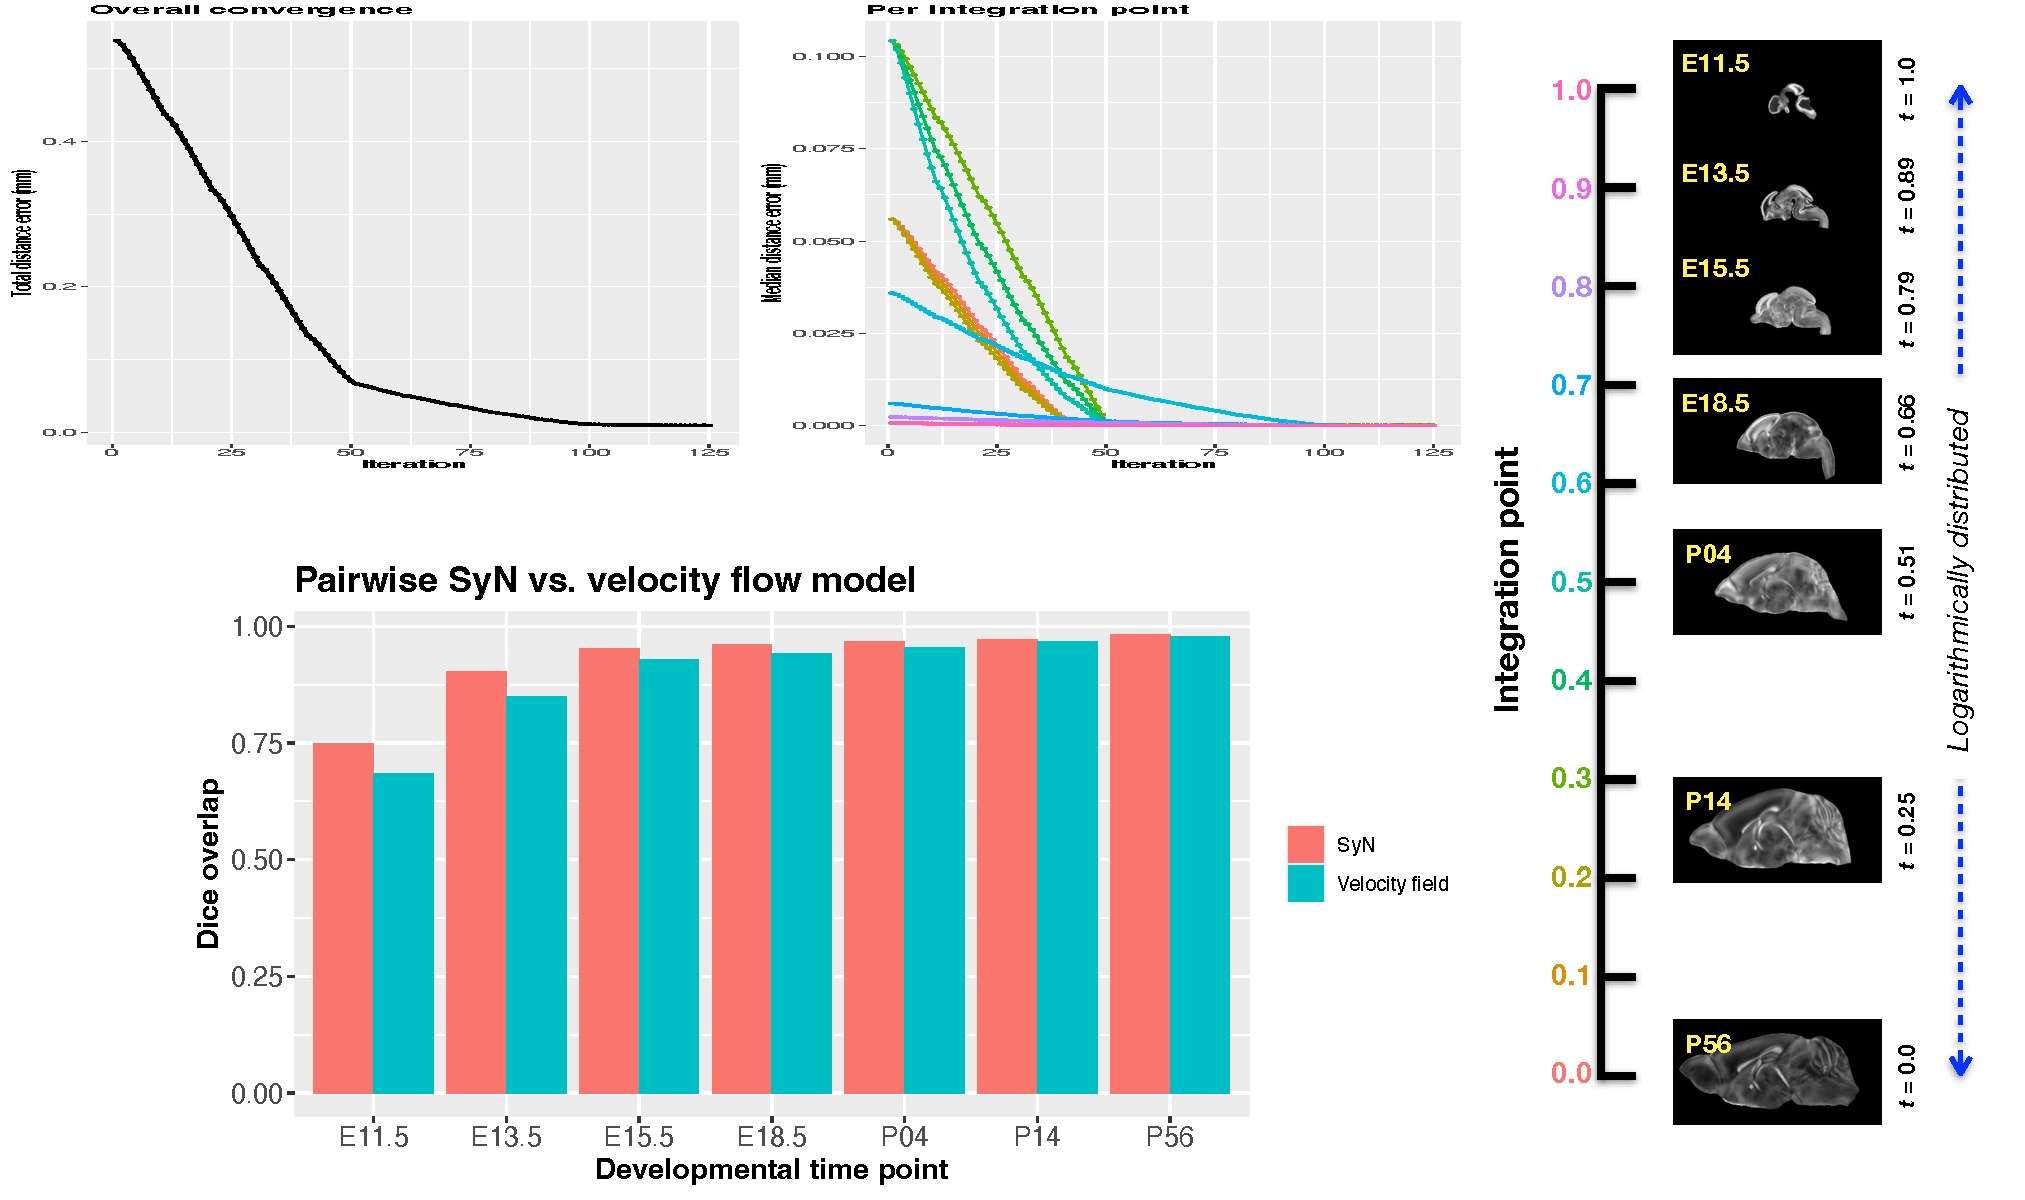
\includegraphics[width=0.99\textwidth]{Figures/convergence.pdf}
\caption{Convergence and evaluation of the velocity flow model across the
DevCCF developmental trajectory. (Top left) Total displacement error over
iterations. (Top right) Median displacement error per integration point across
the optimization timeline, spanning embryonic (E11.5) to postnatal (P56) stages.
(Bottom) Dice similarity scores comparing region-level label overlap between:
(1) conventional pairwise SyN registration and (2) velocity flow-based
deformation, across intermediate timepoints. Using region-based pairwise
registration with SyN as a performance upper bound, the velocity flow model
achieves comparable accuracy while also enabling smooth, continuous deformation
across the full developmental continuum.}
\label{fig:convergence}
\end{figure}

The velocity field was optimized using the seven corresponding point
sets and their associated weights. The field geometry was defined at
\([256, 182, 360]\) with 11 integration points at 50 \(\mu\)m
resolution, yielding a compressed velocity model of \(\sim2\) GB. This
resolution balanced accuracy and computational tractability while
remaining portable. All data and code are publicly available in the
accompanying GitHub repository.

To normalize temporal spacing, we assigned scalar values in \([0, 1]\)
to each template. Given the nonlinear spacing in postnatal development,
we applied a logarithmic transform to the raw time values prior to
normalization. Within this logarithmic temporal transform, P56 was
assigned a span of 28 postnatal days to reflect known developmental
dynamics (i.e., in terms of modeling the continuous deformation, the
morphological changes between Day 28 and Day 56 are insignificant). This
improved the temporal distribution of integration points (Figure
\ref{fig:convergence}, right panel).

Optimization was run for a maximum of 200 iterations using a 2020 iMac
(3.6 GHz 10-Core Intel Core i9, 64 GB RAM), with each iteration taking
\(\sim6\) minutes. During each iteration, the velocity field was updated
across all 11 integration points by computing regularized displacement
fields between warped point sets at adjacent time slices. Updates were
applied using a step size of \(\delta = 0.2\). Convergence was assessed
via average displacement error across all points, with final convergence
achieved after \(\sim125\) iterations (Figure \ref{fig:convergence},
left panel). Median errors across integration points also trended toward
zero, albeit at varying rates. To benchmark performance, we compared the
velocity model's region-based alignment to traditional pairwise
registration using SyN, a widely used diffeomorphic algorithm. The
velocity model achieved comparable Dice scores at sampled timepoints
while additionally offering smooth interpolation across the entire
developmental trajectory.

\subsubsection{The velocity flow transformation
model}\label{the-velocity-flow-transformation-model}

\begin{figure}[!htb]
\centering
\includegraphics[width=0.8\textwidth]{Figures/CrossWarp.pdf}
\caption{Mid-sagittal visualization of DevCCF templates warped to every other time point. Each row is a reference space; each column is a warped input. Diagonal entries show original templates.}
\label{fig:crosswarp}
\end{figure}

\begin{figure}[!htb]
\centering
\includegraphics[width=0.8\textwidth]{Figures/pseudo_template.pdf}
\caption{Example of generating “virtual” DevCCF templates at intermediate time points (e.g., P10.3, P20) by warping adjacent stages to a shared time and averaging using ANTsX.}
\label{fig:virtual}
\end{figure}

Once optimized, the velocity field enables the computation of
diffeomorphic transformations between any pair of continuous time points
within the DevCCF developmental range. Figure\,\ref{fig:crosswarp}
illustrates cross-warping between all DevCCF stages using the velocity
flow model. In addition to facilitating flexible alignment between
existing templates, the model also supports the synthesis of virtual
templates at intermediate, unsampled developmental stages. As shown in
Figure\,\ref{fig:virtual}, we demonstrate the creation of virtual age
templates (e.g., P10.3 and P20) by warping adjacent developmental
atlases to a target timepoint and constructing an averaged
representation using ANTsX's template-building functionality.

All usage examples, scripts, and supporting data for full
reproducibility are publicly available in the associated codebase.

\subsection{Automated structural labeling of the mouse
brain}\label{automated-structural-labeling-of-the-mouse-brain}

\begin{figure}
\centering
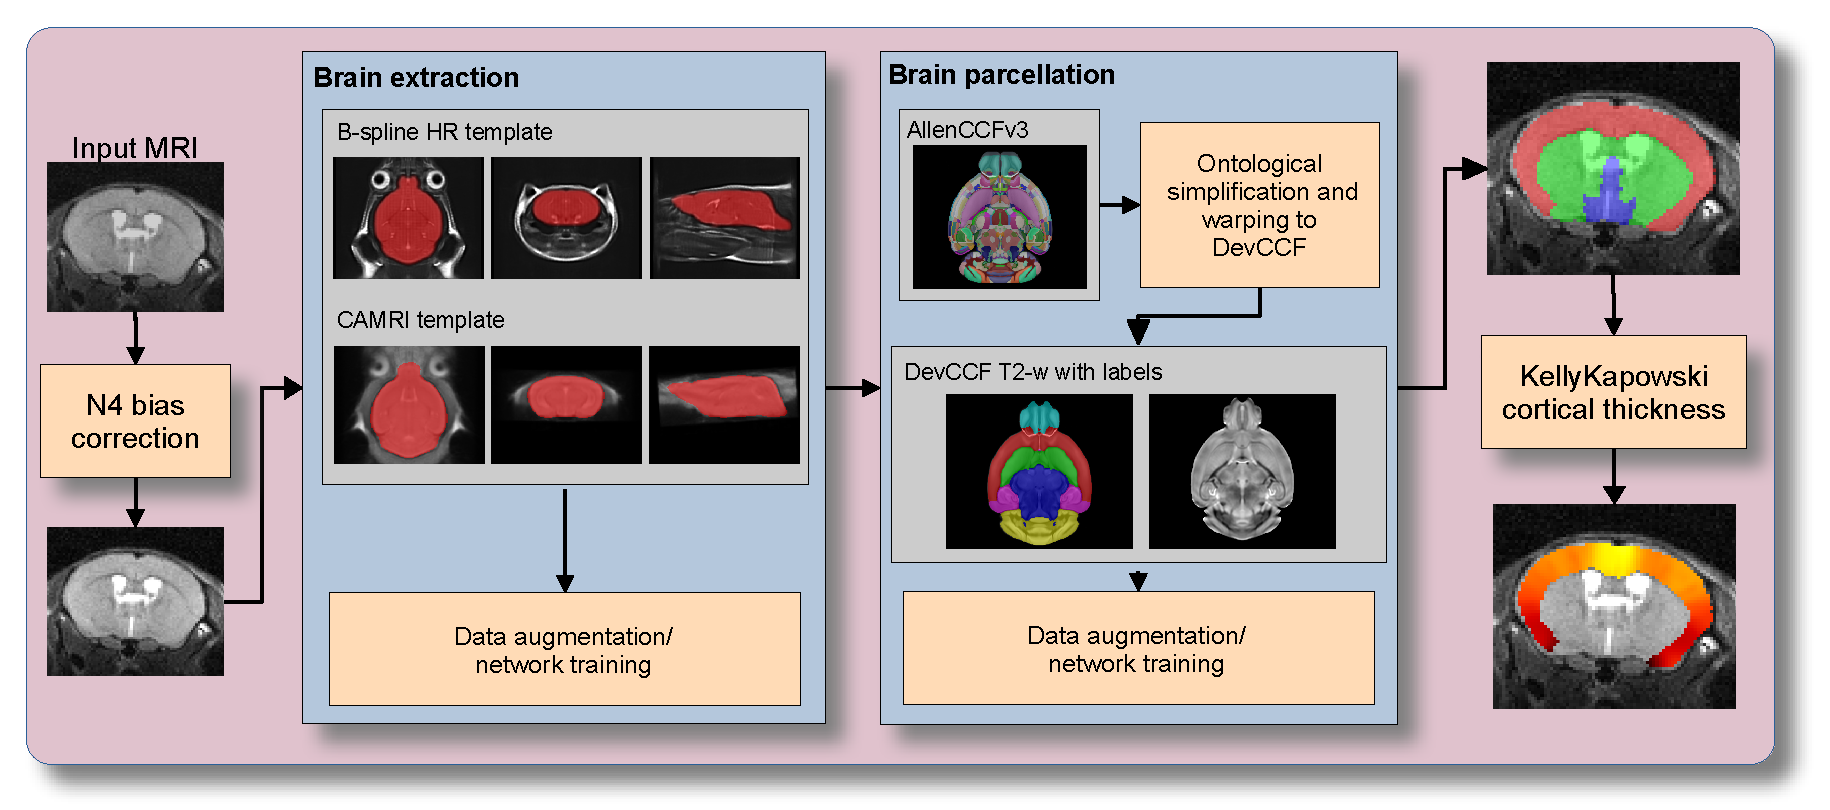
\includegraphics[width=0.95\textwidth]{Figures/mousePipeline.pdf} \caption{The
mouse brain cortical labeling pipeline integrates two deep learning components
for brain extraction and anatomical region segmentation. Both networks rely
heavily on data augmentation applied to templates constructed from open
datasets. The framework also supports further refinement or alternative label
sets tailored to specific research needs. Possible applications include
voxelwise cortical thickness estimation.}
\label{fig:mouseKK}
\end{figure}

Structural labeling strategies for the mouse brain are essential for
understanding the organization and function of the murine nervous
system\textsuperscript{82}. By dividing the brain into anatomically or
functionally defined regions, researchers can localize biological
processes, relate regional features to behavior, or quantify spatial
variation in gene expression patterns\textsuperscript{83,84}. While deep
learning techniques have yielded robust segmentation and labeling tools
for the human brain (e.g., SynthSeg\textsuperscript{85},
ANTsXNet\textsuperscript{45}), analogous development for mouse data
(e.g., MEMOS\textsuperscript{86}) has been limited. Mouse neuroimaging
often presents unique challenges, such as highly anisotropic sampling,
that complicate transfer of existing tools. At the same time, high
resolution resources like the AllenCCFv3 and DevCCF provide reference
label sets that can serve as training data. We demonstrate how ANTsX can
be used to construct a full structural labeling pipeline for the mouse
brain (Figure\,\ref{fig:mouseKK}), including both whole brain
segmentation (i.e., brain extraction) and the subsequent template-based
region segmentation.

\subsubsection{Template-based mouse brain extraction
network}\label{template-based-mouse-brain-extraction-network}

To develop a general-purpose mouse brain extraction model, we
constructed whole-head templates from two publicly available T2-weighted
datasets. The first dataset, from the Center for Animal MRI (CAMRI) at
the University of North Carolina at Chapel Hill\textsuperscript{68},
includes 16 isotropic MRI volumes acquired at
\(0.16 \times 0.16 \times 0.16\) mm\(^3\) resolution. The second
dataset\textsuperscript{69} comprises 88 specimens acquired in three
orthogonal 2D views (coronal, axial, sagittal) at \(0.08 \times 0.08\)
mm\(^3\) in-plane resolution with 0.5 mm slice thickness. These
orthogonal 2D acquisitions were reconstructed into high-resolution 3D
volumes using a B-spline fitting algorithm\textsuperscript{87}. Using
this synthesized dataset and the CAMRI images, we created two
ANTsX-based population templates\textsuperscript{59}, each paired with a
manually delineated brain mask. These served as the basis for training
an initial template-based brain extraction model. Deep learning training
of the network employed aggressive data augmentation strategies,
including bias field simulation, histogram warping, random spatial
deformation, noise injection, and anisotropic resampling. This enabled
the model to generalize beyond the two templates. The initial model was
released through ANTsXNet and made publicly available.

Subsequent community use led to further improvements. A research group
applying the tool to their own ex vivo T2-weighted mouse brain data
contributed a third template and associated mask (acquired at 0.08 mm
isotropic resolution). Incorporating this into the training data
improved robustness and accuracy to an independent dataset and extended
the model's generalizability. The refined model is distributed through
ANTsPyNet via \texttt{antspynet.mouse\_brain\_extraction(...)}.

\subsubsection{Template-based mouse brain anatomical
labeling}\label{template-based-mouse-brain-anatomical-labeling}

The AllenCCFv3 atlas and its hierarchical ontology, along with the
DevCCF, provide a strong foundation for developing region-wise
anatomical labeling models for multi-modal mouse brain imaging. Using
the \texttt{allensdk} Python library, we generated a coarse segmentation
scheme by grouping anatomical labels into six major regions: cerebral
cortex, cerebral nuclei, brainstem, cerebellum, main olfactory bulb, and
hippocampal formation. These labels were mapped onto the P56 T2-weighted
DevCCF template to serve as training targets. We trained a 3D
U-net--based segmentation network using this template and the same
augmentation strategies described for brain extraction. The model is
publicly available via ANTsXNet
(\texttt{antspynet.mouse\_brain\_parcellation(...)}) and supports robust
anatomical labeling across diverse imaging geometries and contrasts. The
inclusion of aggressive augmentation, including simulated anisotropy,
enables the model to perform well even on thick-slice input data.
Internally, the model reconstructs isotropic probability and label maps,
facilitating downstream morphometric analyses. For example, this network
integrates with the ANTsX cortical thickness estimation pipeline
(\texttt{antspynet.mouse\_cortical\_thickness(...)}) to produce
voxelwise cortical thickness maps, even when applied to anisotropic or
limited-resolution mouse brain data.

\subsubsection{Evaluation}\label{evaluation}

\begin{figure}
\centering
  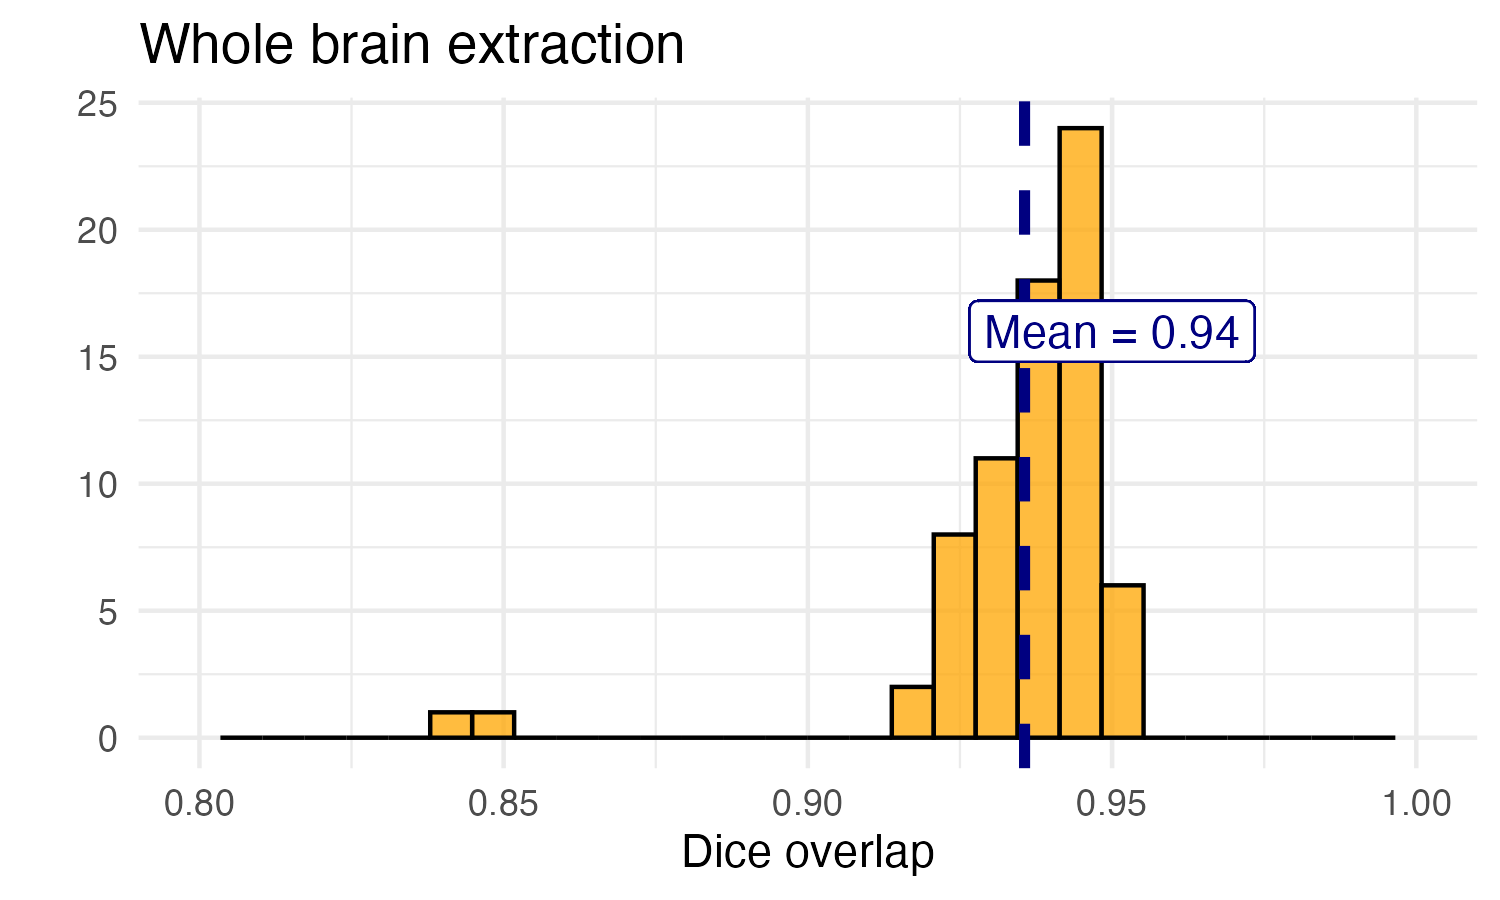
\includegraphics[width=0.75\textwidth]{Figures/diceWholeBrain.png}
\caption{Evaluation of the ANTsX mouse brain extraction on an
independent, publicly available dataset consisting of 12 specimens $\times$ 7
time points = 84 total images.  Dice overlap comparisons with the
user-generated brain masks provide good agreement with the automated results
from the brain extraction network.}
\label{fig:evaluation}
\end{figure}

\begin{figure}
\centering
\begin{subfigure}{0.25\textwidth}
  \centering
  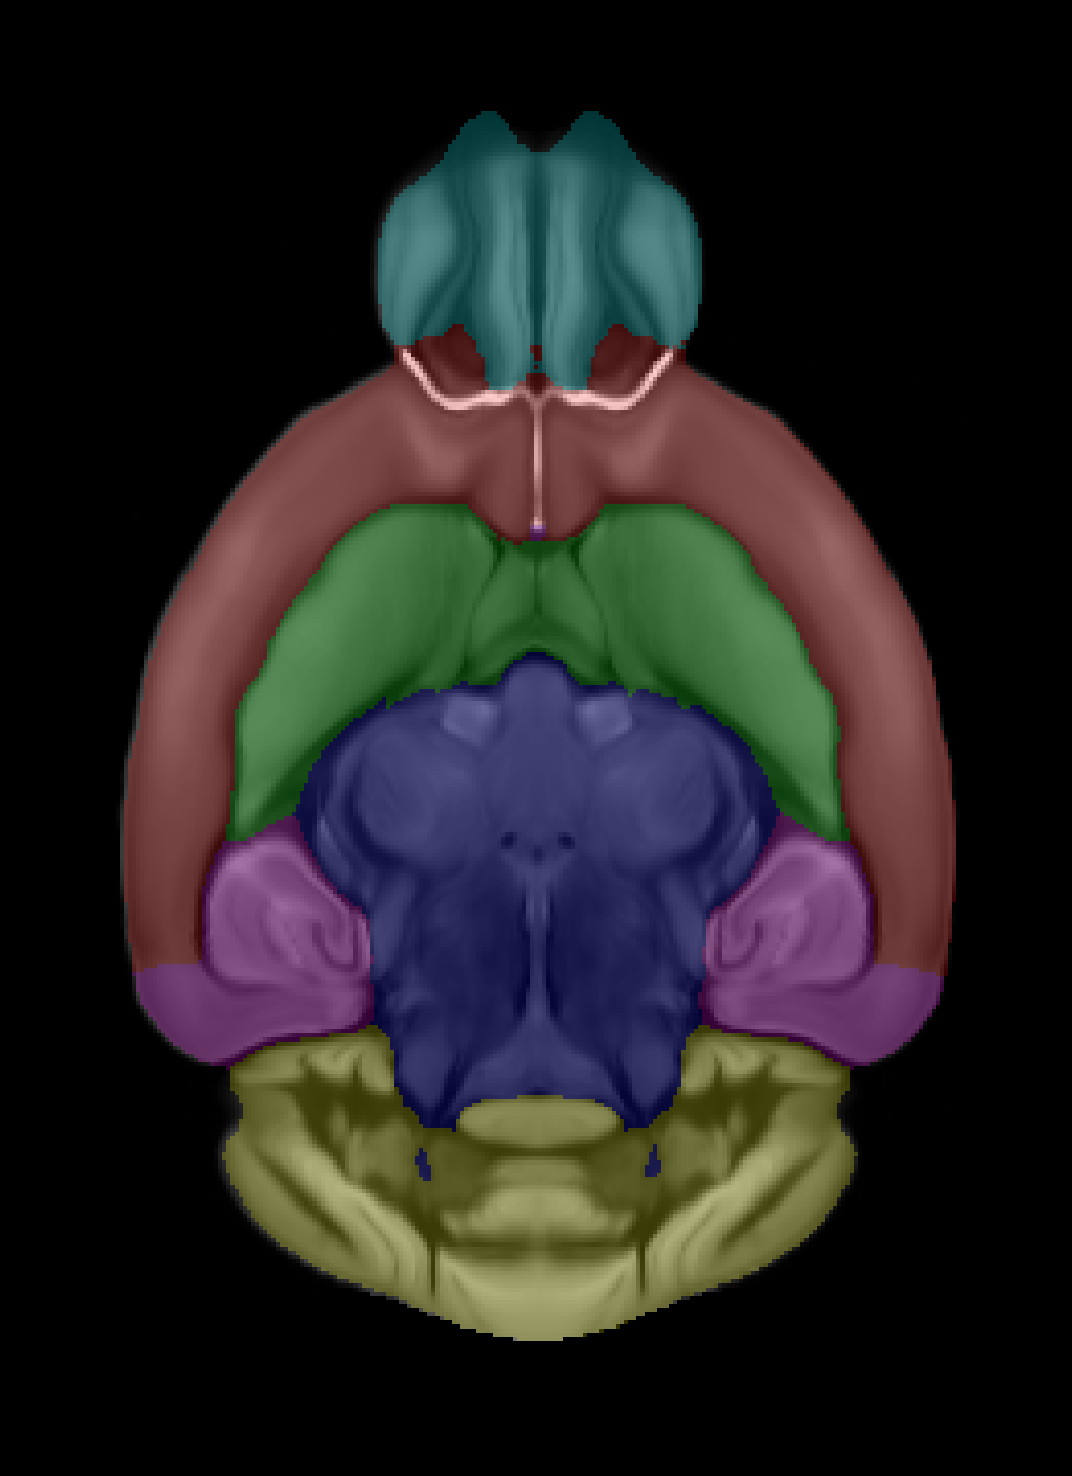
\includegraphics[width=\linewidth]{Figures/AllenCCFv3_parcellation_slice91.png}
  \caption{}
  \label{fig:subp_a}
\end{subfigure}
\begin{subfigure}{0.25\textwidth}
  \centering
  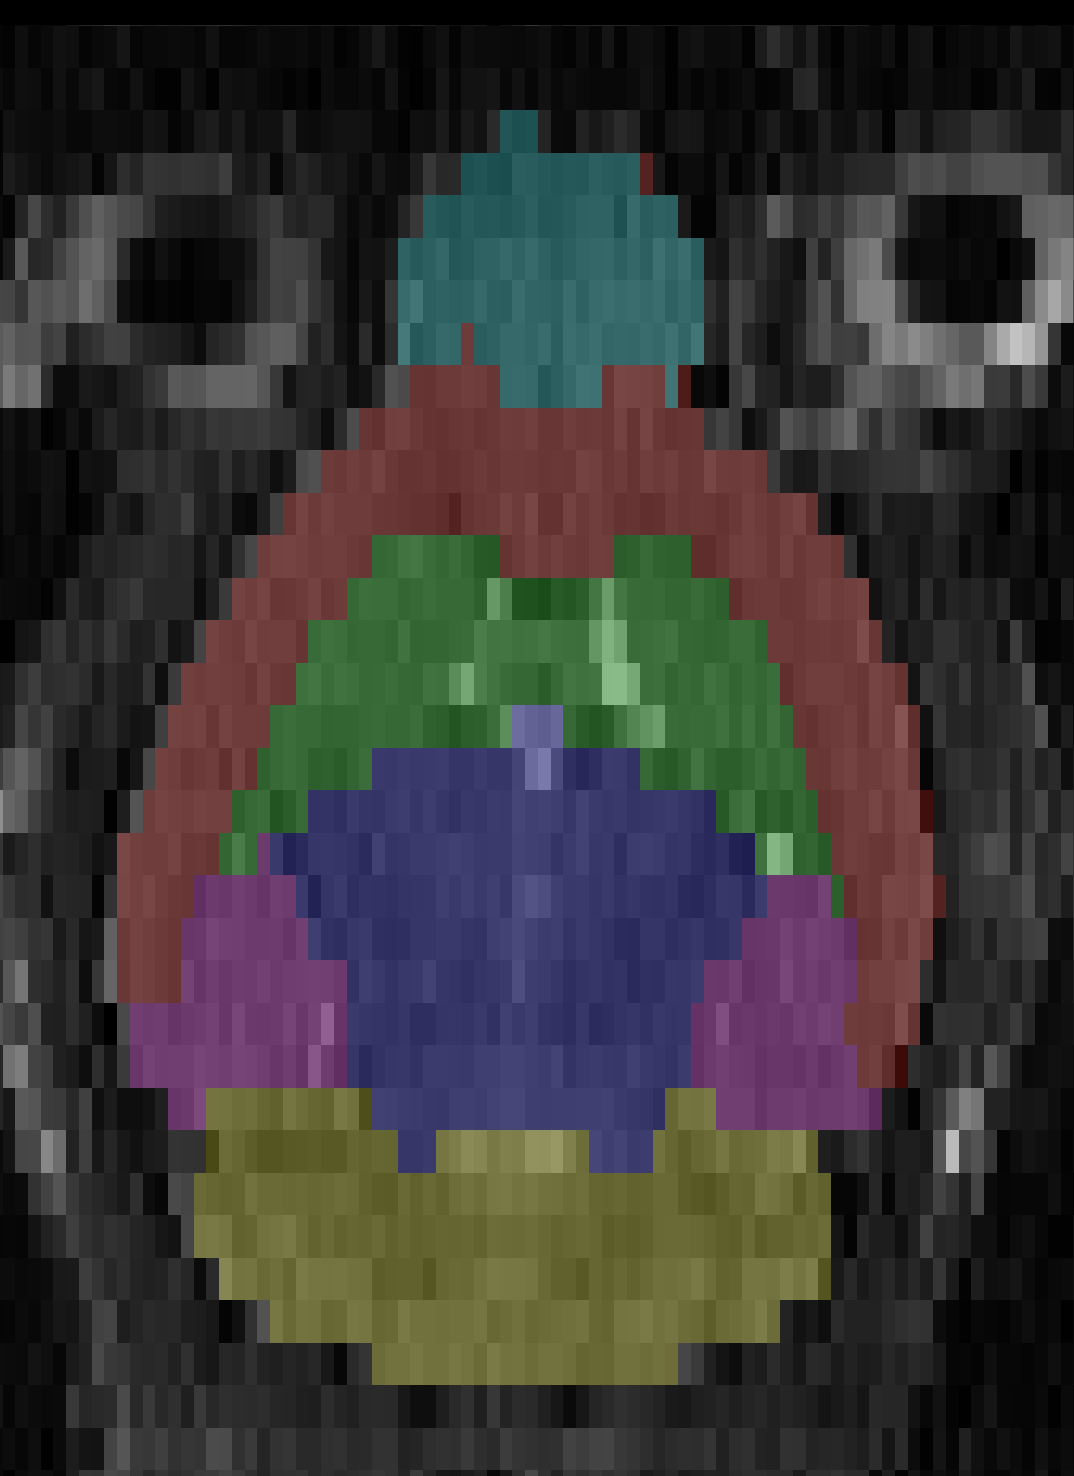
\includegraphics[width=\linewidth]{Figures/NR5_M_Day0_slice53.png}
  \caption{}
  \label{fig:subp_b}
\end{subfigure} \\
\begin{subfigure}{.75\textwidth}
  \centering
  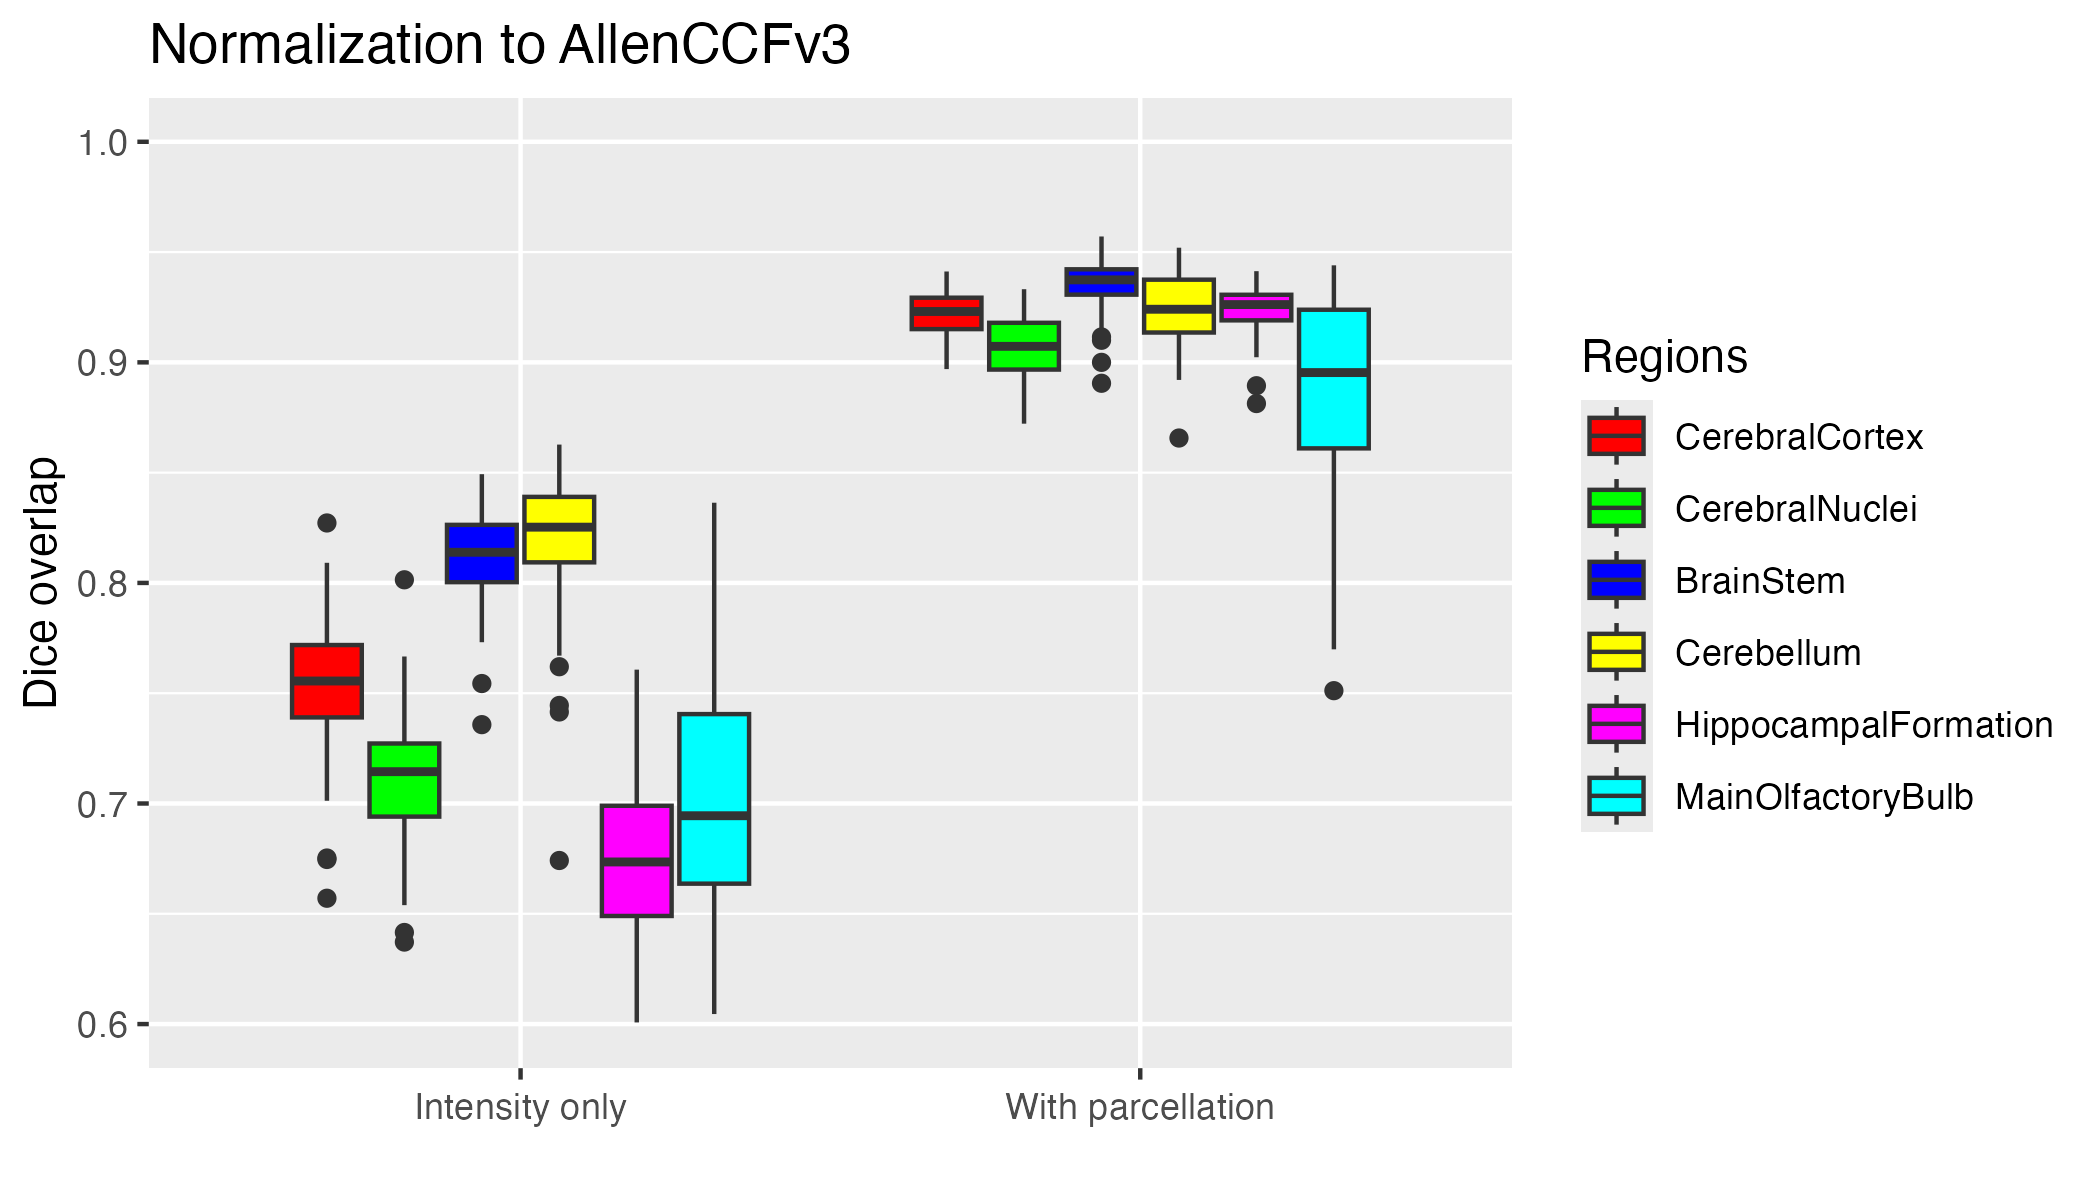
\includegraphics[width=\linewidth]{Figures/diceAllenCCFv3.png}
  \caption{}
  \label{fig:subc}
\end{subfigure}
\caption{Evaluation of the ANTsX deep learning–based mouse brain parcellation on
a diverse MRI cohort. (a) T2-weighted DevCCF P56 template with the six-region
parcellation: cerebral cortex, nuclei, brain stem, cerebellum, main olfactory
bulb, and hippocampal formation. (b) Example segmentation result from a
representative subject (NR5, Day 0) using the proposed deep learning pipeline.
(c) Dice overlap scores across the full evaluation cohort ($n=84$), comparing
anatomical alignment achieved via registration using intensity alone versus
registration guided by the predicted parcellation. Dice values were computed
using manually segmented labels transformed to AllenCCFv3 space.}
\label{fig:evaluationParcellation}
\end{figure}

For evaluation, we used an additional publicly available
dataset\textsuperscript{70} that is completely independent from the data
used in training the brain extraction and parcellation networks. Data
includes 12 specimens each imaged at seven time points (Day 0, Day 3,
Week 1, Week 4, Week 8, Week 20) with in-house-generated brain masks
(i.e., produced by the data providers) for a total of 84 images. Spacing
is anistropic with an in-plane resolution of \(0.1 \times 0.1\) mm\(^2\)
and a slice thickness of \(0.5\) mm.

Figure\,\ref{fig:evaluation} summarizes the whole-brain overlap between
manually segmented reference masks and the predicted segmentations for
all 84 images in the evaluation cohort. The proposed network
demonstrates excellent performance in brain extraction across a wide age
range. To further assess the utility of the parcellation network, we
used the predicted labels to guide anatomically informed registration to
the AllenCCFv3 atlas using ANTsX multi-component registration, and
compared this to intensity-only registration
(Figure\,\ref{fig:evaluationParcellation}). While intensity-based
alignment performs reasonably well, incorporating the predicted
parcellation significantly improves regional correspondence. Dice scores
shown in Figure\,\ref{fig:evaluationParcellation}(c) were computed using
manually segmented labels transformed to AllenCCFv3 space. \clearpage
\newpage

\section{Discussion}\label{discussion}

The diverse mouse brain cell type profiles gathered through BICCN and
associated efforts provide a rich multi-modal resource to the research
community. However, despite significant progress, optimal leveraging of
these valuable resources remains an ongoing challenge. A central
component to data integration is accurately mapping novel cell type data
into common coordinate frameworks (CCFs) for subsequent processing and
analysis. To meet these needs, tools for mapping mouse brain data must
be both broadly accessible and capable of addressing challenges unique
to each modality. In this work, we described modular ANTsX-based
pipelines developed to support three distinct BICCN efforts encompassing
spatial transcriptomic, morphological, and developmental data. We
demonstrated how a flexible image analysis toolkit like ANTsX can be
tailored to address specific modality-driven constraints by leveraging
reusable, validated components.

As part of collaborative efforts with the Allen Institute for Brain
Science and the broader BICCN initiative, we developed two modular
pipelines for mapping MERFISH and fMOST datasets to the AllenCCFv3.
These workflows were designed to accommodate the specific requirements
of high-resolution transcriptomic and morphological data while
leveraging reusable components from the ANTsX ecosystem. The MERFISH
pipeline incorporates preprocessing and registration steps tailored to
known anatomical and imaging artifacts in multiplexed spatial
transcriptomic data. While the general mapping strategy is applicable to
other sectioned histological datasets, these refinements demonstrate how
general-purpose tools can be customized to meet the demands of
specialized modalities. The fMOST workflow, in contrast, emphasizes
reusability and consistency across large datasets. It introduces an
intermediate, canonical fMOST atlas to stabilize transformations to the
AllenCCFv3, reducing the need for repeated manual alignment and enabling
standardized mapping of single-neuron reconstructions to a common
coordinate framework.

Evaluation of both workflows followed established QA/QC protocols used
at the Allen Institute, emphasizing biologically meaningful criteria
such as expected gene-marker alignment (MERFISH) and accurate
reconstruction of neuronal morphology (fMOST). These domain-informed
assessments, also used in prior large-scale mapping
projects\textsuperscript{46}, prioritize task-relevant accuracy over
other possible benchmarks such as Dice coefficients or landmark
distances. While formal quantitative scores were not reported for these
specific pipelines, they both demonstrate reliable, expert-validated
performance in collaborative contexts. Additional documentation and
evaluation commentary are available in the updated CCFAlignmentToolkit
GitHub repository.

For developmental data, we introduced a velocity field--based model for
continuous interpolation between discrete DevCCF timepoints. Although
the DevCCF substantially expands coverage of developmental stages
relative to prior atlases, temporal gaps remain. The velocity model
enables spatio-temporal transformations within the full developmental
interval and supports the generation of virtual templates at unsampled
ages. This functionality is built using ANTsX components for velocity
field optimization and integration, and offers a novel mechanism for
interpolating across the non-linear developmental trajectory of the
mouse brain. Such interpolation has potential utility for both
anatomical harmonization and longitudinal analyses. Interestingly,
long-range transformations (e.g., P56 to E11.5) revealed anatomy
evolving in plausible ways yet sometimes diverging from known
developmental patterns (e.g., hippocampal shape changes) reflecting the
input data and offering insight into temporal gaps. These behaviors
could assist future efforts to determine which additional time points
would most improve spatiotemporal coverage.

We also introduced a template-based deep learning pipeline for mouse
brain extraction and parcellation using aggressive data augmentation.
This approach is designed to reduce the reliance on large annotated
training datasets, which remain limited in the mouse imaging domain.
Evaluation on independent data demonstrates promising generalization,
though further refinement will be necessary. As with our human-based
ANTsX pipelines, failure cases can be manually corrected and recycled
into future training cycles. Community contributions are welcomed and
encouraged, providing a pathway for continuous improvement and
adaptation to new datasets.

The ANTsX ecosystem offers a powerful foundation for constructing
scalable, reproducible pipelines for mouse brain data analysis. Its
modular design and multi-platform support enable researchers to develop
customized workflows without extensive new software development. The
widespread use of ANTsX components across the neuroimaging community
attests to its utility and reliability. As a continuation of the BICCN
program, ANTsX is well positioned to support the goals of the BRAIN
Initiative Cell Atlas Network (BICAN) and future efforts to extend these
mapping strategies to the human brain.

\clearpage \newpage

\section{Methods}\label{methods}

The following methods are all available as part of the ANTsX ecosystem
with analogous elements existing in both ANTsR (ANTs in R) and ANTsPy
(ANTs in Python), underpinned by a shared ANTs/ITK C++ core. Most
development for the work described was performed using ANTsPy. For
equivalent functionality in ANTsR, we refer the reader to the
comprehensive ANTsX tutorial: \url{https://tinyurl.com/antsxtutorial}.

\subsection{General ANTsX utilities}\label{general-antsx-utilities}

Although focused on distinct data types, the three pipelines presented
in this work share common components that address general challenges in
mapping mouse brain data. These include correcting image intensity
artifacts, denoising, spatial registration, template generation, and
visualization. Table \ref{table:methods} provides a concise summary of
the relevant ANTsX functionality.


\begin{table}
  \small
   \centering
   \vspace{-0.25cm}
   \caption{Sampling of ANTsX functionality} 
   \begin{tabular*}{0.95\textwidth}{l @{\extracolsep{\fill}} p{.575\textwidth}}
    \toprule
    \multicolumn{2}{c}{\cellcolor{gray!25} \em ANTsPy: Preprocessing} \\
    \cmidrule[1pt](lr){1-2}
    bias field correction & \texttt{n4\_bias\_field\_correction(...)} \\
    image denoising  & \texttt{denoise\_image(...)} \\
    \cmidrule[1pt](lr){1-2}
    \multicolumn{2}{c}{\cellcolor{gray!25} \em ANTsPy: Registration} \\
    \cmidrule[1pt](lr){1-2}
    image registration & \texttt{registration(...)} \\
    image transformation & \texttt{apply\_transforms(...)} \\
    template generation  & \texttt{build\_template(...)} \\
    landmark registration & \texttt{fit\_transform\_to\_paired\_points(...)} \\
    time-varying landmark reg. & \texttt{fit\_time\_varying\_transform\_to\_point\_sets(...)} \\
    integrate velocity field & \texttt{integrate\_velocity\_field(...)} \\
    invert displacement field & \texttt{invert\_displacement\_field(...)} \\
    \cmidrule[1pt](lr){1-2}
    \multicolumn{2}{c}{\cellcolor{gray!25} \em ANTsPy: Segmentation} \\
    \cmidrule[1pt](lr){1-2}
    MRF-based segmentation & \texttt{atropos(...)} \\
    Joint label fusion & \texttt{joint\_label\_fusion(...)} \\
    diffeormorphic thickness   & \texttt{kelly\_kapowski(...)} \\
    \cmidrule[1pt](lr){1-2}
    \multicolumn{2}{c}{\cellcolor{gray!25} \em ANTsPy: Miscellaneous} \\
    \cmidrule[1pt](lr){1-2}
    Regional intensity statistics & \texttt{label\_stats(...)} \\
    Regional shape measures & \texttt{label\_geometry\_measures(...)} \\
    B-spline approximation & \texttt{fit\_bspline\_object\_to\_scattered\_data(...)} \\
    Visualize images and overlays\,\,\,\,\,\,\,\,\,\,\,\, & \texttt{plot(...)} \\
    \cmidrule[1pt](lr){1-2}
    \multicolumn{2}{c}{\cellcolor{gray!25} \em ANTsPyNet: Mouse-specific} \\
    \cmidrule[1pt](lr){1-2}
    brain extraction & \texttt{mouse\_brain\_extraction(...modality="t2"...)} \\
    brain parcellation & \texttt{mouse\_brain\_parcellation(...)}  \\
    cortical thickness & \texttt{mouse\_cortical\_thickness(...)}  \\
    % foreground extraction & \texttt{mouse\_histology\_brain\_mask(...)} \\
    % midline segmentation & \texttt{mouse\_histology\_hemispherical\_coronal\_mask(...)} \\
    % cerebellum segmentation & \texttt{mouse\_histology\_cerebellum\_mask(...)} \\
    super resolution & \texttt{mouse\_histology\_super\_resolution(...)} \\
    \bottomrule
    \multicolumn{2}{l}{\makecell[l]{
     \vspace{-3pt}
     \scriptsize ANTsX provides state-of-the-art functionality for processing biomedical image data.  Such tools, including deep \\
     \vspace{-3pt}
     \scriptsize learning networks, support a variety of mapping-related tasks.  A more comprehensive listing of ANTsX tools with \\
     \vspace{-3pt}
     \scriptsize self-contained R and Python examples is provided as a gist page on GitHub (\url{https://tinyurl.com/antsxtutorial}). }
    }
   \end{tabular*}
 \label{table:methods}
\end{table}


\textbf{Preprocessing: bias field correction and denoising.} Standard
preprocessing steps in mouse brain imaging include correcting for
spatial intensity inhomogeneities and reducing image noise, both of
which can impact registration accuracy and downstream analysis. ANTsX
provides implementations of widely used methods for these tasks. The N4
bias field correction algorithm\textsuperscript{51}, originally
developed in ANTs and contributed to ITK, mitigates artifactual,
low-frequency intensity variation and is accessible via
\texttt{ants.n4\_bias\_field\_correction(...)}. Patch-based
denoising\textsuperscript{61} has been implemented as
\texttt{ants.denoise\_image(...)}.

\textbf{Image registration.} ANTsX includes a robust and flexible
framework for pairwise and groupwise image
registration\textsuperscript{81}. At its core is the SyN
algorithm\textsuperscript{50}, a symmetric diffeomorphic model with
optional B-spline regularization\textsuperscript{67}. In ANTsPy,
registration is performed via \texttt{ants.registration(...)} using
preconfigured parameter sets (e.g.,
\texttt{antsRegistrationSyNQuick{[}s{]}},
\texttt{antsRegistrationSyN{[}s{]}}) suitable for different imaging
modalities and levels of computational demand. Resulting transformations
can be applied to new images with \texttt{ants.apply\_transforms(...)}.

\textbf{Template generation.} ANTsX supports population-based template
generation through iterative pairwise registration to an evolving
estimate of the mean shape and intensity reference space across
subjects\textsuperscript{59}. This functionality was used in generating
the DevCCF templates\textsuperscript{16}. The procedure, implemented as
\texttt{ants.build\_template(...)}, produces average images in both
shape and intensity by aligning all inputs to a common evolving
template.

\textbf{Visualization.} To support visual inspection and quality
control, ANTsPy provides flexible image visualization with
\texttt{ants.plot(...)}. This function enables multi-slice and
multi-orientation rendering with optional overlays and label maps.

\subsection{Mapping fMOST data to
AllenCCFv3}\label{mapping-fmost-data-to-allenccfv3}

\textbf{Preprocessing.} Mapping fMOST data into the AllenCCFv3 presents
unique challenges due to its native ultra-high resolution and imaging
artifacts common to the fMOST modality. Each fMOST image can exceed a
terabyte in size, with spatial resolutions far exceeding those of the
AllenCCFv3 (25\,\(\mu m\) isotropic). To reduce computational burden and
prevent resolution mismatch, each fMOST image is downsampled using cubic
B-spline interpolation via \texttt{ants.resample\_image(...)} to match
the template resolution.

Stripe artifacts (i.e., periodic intensity distortions caused by
nonuniform sectioning or illumination) are common in fMOST and can
mislead deformable registration algorithms. These were removed using a
custom 3D notch filter (\texttt{remove\_stripe\_artifact(...)})
implemented in the \texttt{CCFAlignmentToolkit} using SciPy frequency
domain filtering. The filter targets dominant stripe frequencies along a
user-specified axis in the Fourier domain. In addition, intensity
inhomogeneity across sections, often arising from variable staining or
illumination, was corrected using N4 bias field correction.

\textbf{Template-based spatial normalization.} To facilitate
reproducible mapping, we first constructed a contralaterally symmetric
average template from 30 fMOST brains and their mirrored counterparts
using ANTsX template-building tools. Because the AllenCCFv3 and fMOST
data differ substantially in both intensity contrast and morphology,
direct deformable registration between individual fMOST brains and the
AllenCCFv3 was insufficiently robust. Instead, we performed a one-time
expert-guided label-driven registration between the average fMOST
template and AllenCCFv3. This involved sequential alignment of seven
manually selected anatomical regions: 1) brain mask/ventricles, 2)
caudate/putamen, 3) fimbria, 4) posterior choroid plexus, 5) optic
chiasm, 6) anterior choroid plexus, and 7) habenular commissure which
were prioritized to enable coarse-to-fine correction of shape
differences. Once established, this fMOST-template-to-AllenCCFv3
transform was reused for all subsequent specimens. Each new fMOST brain
was then registered to the average fMOST template using intensity-based
registration, followed by concatenation of transforms to produce the
final mapping into AllenCCFv3 space.

\textbf{Mapping neuron projections.} A key advantage of fMOST imaging is
its ability to support single neuron projection reconstruction across
the entire brain\textsuperscript{78}. Because these reconstructions are
stored as 3D point sets aligned to the original fMOST volume, we applied
the same composite transform used for image alignment to the point data
using ANTsX functionality. This enables seamless integration of cellular
morphology data into AllenCCFv3 space, facilitating comparative analyses
across specimens.

\subsection{Mapping MERFISH data to
AllenCCFv3}\label{mapping-merfish-data-to-allenccfv3}

\textbf{Preprocessing.} MERFISH data are acquired as a series of 2D
tissue sections, each comprising spatially localized gene expression
measurements at subcellular resolution. To enable 3D mapping to the
AllenCCFv3, we first constructed anatomical reference images by
aggregating the number of detected transcripts per voxel across all
probes within each section. These 2D projections were resampled to a
resolution of 10 \(\mu m\)\,\(\times\)\,10\,\(\mu m\) to match the
in-plane resolution of the AllenCCFv3.

Sections were coarsely aligned using manually annotated dorsal and
ventral midline points, allowing initial volumetric reconstruction.
However, anatomical fidelity remained limited by variation in section
orientation, spacing, and tissue loss. To further constrain alignment
and enable deformable registration, we derived region-level anatomical
labels directly from the gene expression data.

\textbf{Label creation.} To assign region labels to the MERFISH data, we
use a cell type clustering approach previously
detailed\textsuperscript{46}. In short, manually dissected scRNAseq data
was used to establish the distribution of cell types present in each of
the following major regions: cerebellum, CTXsp, hindbrain, HPF,
hypothalamus, isocortex, LSX, midbrain, OLF, PAL, sAMY, STRd, STRv,
thalamus and hindbrain. Clusters in the scRNA-seq dataset were then used
to assign similar clusters of cell types in the MERFISH data to the
regions they are predominantly found in the scRNA-seq data. To account
for clusters that were found at low frequency in regions outside its
main region we calculated for each cell its 50 nearest neighbors in
physical space and reassigned each cell to the region annotation
dominating its neighborhood.

\textbf{Section matching via global alignment.} A major challenge was
compensating for oblique cutting angles and non-uniform section
thickness, which distort the anatomical shape and spacing of the
reconstructed volume. Rather than directly warping the MERFISH data into
atlas space, we globally aligned the AllenCCFv3 to the MERFISH
coordinate system. This was done via an affine transformation followed
by resampling of AllenCCFv3 sections to match the number and orientation
of MERFISH sections. This approach minimizes interpolation artifacts in
the MERFISH data and facilitates one-to-one section matching.

\textbf{Landmark-driven deformable alignment.} We used a 2.5D approach
for fine alignment of individual sections. In each MERFISH slice,
deformable registration was driven by sequential alignment of anatomical
landmarks between the label maps derived from MERFISH and AllenCCFv3. A
total of nine regions, including isocortical layers 2/3, 5, and 6, the
striatum, hippocampus, thalamus, and medial/lateral habenula, were
registered in an empirically determined order. After each round,
anatomical alignment was visually assessed by an expert, and the next
structure was selected to maximize improvement in the remaining
misaligned regions.

The final transform for each section combined the global affine
alignment and the per-structure deformable registrations. These were
concatenated to generate a 3D mapping from the original MERFISH space to
the AllenCCFv3 coordinate system. Once established, the composite
mapping enables direct transfer of gene-level and cell-type data from
MERFISH into atlas space, allowing integration with other imaging and
annotation datasets.

\subsection{DevCCF velocity flow transformation
model}\label{devccf-velocity-flow-transformation-model}

The Developmental Common Coordinate Framework
(DevCCF)\textsuperscript{16} provides a discrete set of age-specific
templates that temporally sample the developmental trajectory. To model
this biological progression more continuously, we introduce a velocity
flow--based paradigm for inferring diffeomorphic transformations between
developmental stages. This enables anatomically plausible estimation of
intermediate templates or mappings at arbitrary timepoints between the
E11.5 and P56 endpoints of the DevCCF. Our approach builds on
established insights from time-varying diffeomorphic
registration\textsuperscript{66}, where a velocity field governs the
smooth deformation of anatomical structures over time. Importantly, the
framework is extensible and can naturally accommodate additional
timepoints for the potential expansion of the DevCCF.

\textbf{Point sampling and region correspondence.} We first coalesced
the anatomical labels across the seven DevCCF templates (E11.5, E13.5,
E15.5, E18.5, P4, P14, P56) into 26 common structures that could be
consistently identified across development. These include major brain
regions such as the cortex, cerebellum, hippocampus, midbrain, and
ventricles. For each successive pair of templates, we performed
multi-label deformable registration using ANTsX to generate forward and
inverse transforms between anatomical label volumes. From the P56 space,
we randomly sampled approximately 1e6 points within and along the
boundaries of each labeled region and propagated them through each
pairwise mapping step (e.g., P56 \(\rightarrow\) P14, P14
\(\rightarrow\) P4, \ldots, E13.5 \(\rightarrow\) E11.5). This procedure
created time-indexed point sets tracing the spatial evolution of each
region.

\textbf{Velocity field fitting.} Using these point sets, we fit a
continuous velocity field over developmental time using a generalized
B-spline scattered data approximation method\textsuperscript{87}. The
field was parameterized over a log-scaled time axis to ensure finer
temporal resolution during early embryonic stages, where morphological
changes are most rapid. Optimization proceeded for approximately 125
iterations, minimizing the average Euclidean norm between transformed
points at each step. Ten integration points were used to ensure
numerical stability. The result is a smooth, differentiable vector field
that defines a diffeomorphic transform between any two timepoints within
the template range.

\textbf{Applications and availability.} This velocity model can be used
to estimate spatial transformations between any pair of developmental
stages---even those for which no empirical template exists---allowing
researchers to create interpolated atlases, align new datasets, or
measure continuous structural changes. It also enables developmental
alignment of multi-modal data (e.g., MRI to LSFM) by acting as a
unifying spatiotemporal scaffold. The underlying components for velocity
field fitting and integration are implemented in ITK, and the complete
workflow is accessible in both ANTsPy
(\texttt{ants.fit\_time\_varying\_transform\_to\_point\_sets(...)}) and
ANTsR. In addition the availability of the DevCCF use case,
self-contained examples and usage tutorials are provided in our public
codebase.

\subsection{Automated brain extraction and parcellation with
ANTsXNet}\label{automated-brain-extraction-and-parcellation-with-antsxnet}

To support template-based deep learning approaches for structural brain
extraction and parcellation, we implemented dedicated pipelines using
the ANTsXNet framework. ANTsXNet comprises open-source deep learning
libraries in both Python (ANTsPyNet) and R (ANTsRNet) that interface
with the broader ANTsX ecosystem and are built on TensorFlow/Keras. Our
mouse brain pipelines mirror existing ANTsXNet tools for human imaging
but are adapted for species-specific anatomical variation, lower SNR,
and heterogeneous acquisition protocols.

\subsubsection{Deep learning training
setup}\label{deep-learning-training-setup}

All network-based approaches were implemented using a standard
U-net\textsuperscript{88} architecture and hyperparameters previously
evaluated in ANTsXNet pipelines for human brain
imaging\textsuperscript{45}. This design follows the `no-new-net'
principle\textsuperscript{89}, which demonstrates that a
well-configured, conventional U-net can achieve robust and competitive
performance across a wide range of biomedical segmentation tasks with
little to no architectural modifications from the original. Both
networks use a 3D U-net architecture implemented in TensorFlow/Keras,
with five encoding/decoding levels and skip connections. The loss
function combined Dice and categorical cross-entropy terms. Training
used a batch size of 4, Adam optimizer with an initial learning rate of
2e-4, and early stopping based on validation loss. Training was
performed on an NVIDIA DGX system (4 \(\times\) Tesla V100 GPUs, 256\,GB
RAM). Model weights and preprocessing routines are shared across
ANTsPyNet and ANTsRNet to ensure reproducibility and language
portability. For both published and unpublished trained networks
available through ANTsXNet, all training scripts and data augmentation
generators are publicly available at
\textbf{\url{https://github.com/ntustison/ANTsXNetTraining}}.

\textbf{Data augmentation.} Robust data augmentation was critical to
generalization across scanners, contrast types, and resolutions. We
applied both intensity- and shape-based augmentation strategies:

\begin{itemize}
\item
  \emph{Intensity augmentations:}

  \begin{itemize}
  \tightlist
  \item
    Gaussian, Poisson, and salt-and-pepper noise:\\
    \texttt{ants.add\_noise\_to\_image(...)}
  \item
    Simulated intensity inhomogeneity via bias field
    modeling\textsuperscript{51}:\\
    \texttt{antspynet.simulate\_bias\_field(...)}
  \item
    Histogram warping to simulate contrast
    variation\textsuperscript{90}:\\
    \texttt{antspynet.histogram\_warp\_image\_intensities(...)}
  \end{itemize}
\item
  \emph{Shape augmentations:}

  \begin{itemize}
  \tightlist
  \item
    Random nonlinear deformations and affine transforms:\\
    \texttt{antspynet.randomly\_transform\_image\_data(...)}
  \item
    Anisotropic resampling across axial, sagittal, and coronal planes:\\
    \texttt{ants.resample\_image(...)}
  \end{itemize}
\end{itemize}

\subsubsection{Brain extraction}\label{brain-extraction}

We originally trained a mouse-specific brain extraction model on two
manually masked T2-weighted templates, generated from public
datasets\textsuperscript{68,69}. One of the templates was constructed
from orthogonal 2D acquisitions using B-spline--based volumetric
synthesis via
\texttt{ants.fit\_bspline\_object\_to\_scattered\_data(...)}. Normalized
gradient magnitude was used as a weighting function to emphasize
boundaries during reconstruction\textsuperscript{87}.

This training strategy provides strong spatial priors despite limited
data by leveraging high-quality template images and aggressive
augmentation to mimic population variability. During the development of
this work, the network was further refined through community engagement.
A user from a U.S.-based research institute applied this publicly
available (but then unpublished) brain extraction tool to their own
mouse MRI dataset. Based on feedback and iterative collaboration with
the ANTsX team, the model was retrained and improved to better
generalize to additional imaging contexts. This reflects our broader
commitment to community-driven development and responsiveness to user
needs across diverse mouse brain imaging scenarios.

The final trained network is available via ANTsXNet through the
function\\
\texttt{antspynet.mouse\_brain\_extraction(...)}. Additionally, both
template/mask pairs are accessible via ANTsXNet. For example, one such
image pair is available via:

\begin{itemize}
\tightlist
\item
  Template:\\
  \texttt{antspynet.get\_antsxnet\_data("bsplineT2MouseTemplate")}
\item
  Brain mask:\\
  \texttt{antspynet.get\_antsxnet\_data("bsplineT2MouseTemplateBrainMask")}
\end{itemize}

\subsubsection{Brain parcellation}\label{brain-parcellation}

For brain parcellation, we trained a 3D U-net model using the DevCCF P56
T2-weighted template and anatomical segmentations derived from
AllenCCFv3. This template-based training strategy enables the model to
produce accurate, multi-region parcellations without requiring
large-scale annotated subject data.

To normalize intensity across specimens, input images were preprocessed
using rank-based intensity normalization
(\texttt{ants.rank\_intensity(...)}). Spatial harmonization was achieved
through affine and deformable alignment of each extracted brain to the
P56 template prior to inference. In addition to the normalized image
input, the network also receives prior probability maps derived from the
atlas segmentations, providing additional spatial context.

This general parcellation deep learning framework has also been applied
in collaboration with other groups pursuing related but distinct
projects. In one case, a model variant was adapted for T2-weighted MRI
using an alternative anatomical labeling scheme; in another, a separate
model was developed for serial two-photon tomography (STPT) with a
different parcellation set. All three models are accessible through a
shared interface in ANTsXNet:
\texttt{antspynet.mouse\_brain\_parcellation(...)}. Ongoing work is
further extending this approach to embryonic mouse brain data. These
independent efforts reflect broader community interest in adaptable
parcellation tools and reinforce the utility of ANTsXNet as a platform
for reproducible, extensible deep learning workflows.

\subsubsection{Evaluation and reuse}\label{evaluation-and-reuse}

To assess model generalizability, both the brain extraction and
parcellation networks were evaluated on an independent longitudinal
dataset comprising multiple imaging sessions with varied acquisition
parameters\textsuperscript{70}. Although each label or imaging modality
required retraining, the process was streamlined by the reusable ANTsX
infrastructure enabled by rapid adaptation with minimal overhead. These
results illustrate the practical benefits of a template-based, low-shot
strategy and modular deep learning framework. All trained models,
associated training scripts, and supporting resources are openly
available and designed for straightforward integration into ANTsX
workflows.

\clearpage

\section*{Data Availability}\label{data-availability}
\addcontentsline{toc}{section}{Data Availability}

The following datasets were used in this study and are publicly
available:

\begin{itemize}
\tightlist
\item
  \textbf{Allen Common Coordinate Framework (AllenCCFv3)}: Available
  from the Allen Institute for Brain Science at
  \url{https://atlas.brain-map.org/atlas}.
\item
  \textbf{Developmental Common Coordinate Framework (DevCCF)} MRI and
  LSFM datasets: Publicly available via the Kim Lab
  \url{https://kimlab.io/home/projects/DevCCF/index.html}.
\item
  \textbf{MERFISH spatial transcriptomics data}: Previously
  published\textsuperscript{46} \url{https://portal.brain-map.org}.
\item
  \textbf{Developmental datasets for brain extraction and segmentation}:

  \begin{itemize}
  \tightlist
  \item
    High-resolution MRI data of brain C57BL/6 and BTBR mice in three
    different anatomical views:
    \url{https://data.mendeley.com/datasets/dz9x23fttt/1}.
  \item
    CAMRI Mouse Brain Data:
    \url{https://openneuro.org/datasets/ds002868/versions/1.0.1}
  \end{itemize}
\item
  \textbf{Evaluation dataset for brain extraction and segmentation}: A
  longitudinal microstructural MRI dataset in healthy C57Bl/6 mice at
  9.4 Tesla
  \url{https://www.frdr-dfdr.ca/repo/dataset/9ea832ad-7f36-4e37-b7ac-47167c0001c1}.
\item
  \textbf{ANTsXNet-pretrained templates and models}: Available through
  ANTsPy at
  \href{https://github.com/ANTsX/ANTsXNet}{https://github.com/ANTsX/ANTsPyNet}.
\end{itemize}

\clearpage

\section*{Code Availability}\label{code-availability}
\addcontentsline{toc}{section}{Code Availability}

All processing pipelines and supporting code are openly available at:

\begin{itemize}
\tightlist
\item
  \url{https://github.com/ntustison/ANTsXMouseBrainMapping} (DevCCF
  velocity model and deep learning parcellation). Also contains the
  text, scripts, and data to reproduce the manuscript (including
  figures).
\item
  \url{https://github.com/dontminchenit/CCFAlignmentToolkit} (MERFISH
  and fMOST workflows)
\end{itemize}

\clearpage

\section*{Inclusion and Ethics
Statement}\label{inclusion-and-ethics-statement}
\addcontentsline{toc}{section}{Inclusion and Ethics Statement}

All imaging data were obtained from publicly available sources that were
collected in accordance with institutional animal care and use committee
protocols and relevant ethical regulations. The authors affirm that all
analyses were conducted using open, reproducible methods and that no
exclusionary criteria were applied based on sex, age, or genetic
background. \clearpage

\section*{Acknowledgments}\label{acknowledgments}
\addcontentsline{toc}{section}{Acknowledgments}

Support for the research reported in this work includes funding from the
National Institute of Biomedical Imaging and Bioengineering
(R01-EB031722) and National Institute of Mental Health (RF1-MH124605,
U24-MH114827, and NIH RF1MH124605 to Y.K.).

We also acknowledge the data contribution of Dr.~Adam Raikes (GitHub
@araikes) of the Center for Innovation in Brain Science at the
University of Arizona for refining the weights of the mouse brain
extraction network.

\clearpage

\section*{Author contributions}\label{author-contributions}
\addcontentsline{toc}{section}{Author contributions}

N.T., M.C., and J.G. wrote the main manuscript text and figures. M.C.,
M.K., R.D., S.S., Q.W., L.G., J.D., C.G., and J.G. developed the Allen
registration pipelines. N.T., F.K., J.G., and Y.K. developed the
time-varying velocity transformation model for the DevCCF. N.T. and M.T.
developed the brain parcellation and cortical thickness methodology. All
authors reviewed the manuscript. \clearpage

\section*{References}\label{references}
\addcontentsline{toc}{section}{References}

\phantomsection\label{refs}
\begin{CSLReferences}{0}{0}
\bibitem[\citeproctext]{ref-Keller:2015aa}
\CSLLeftMargin{1. }%
\CSLRightInline{Keller, P. J. \& Ahrens, M. B.
\href{https://doi.org/10.1016/j.neuron.2014.12.039}{Visualizing
whole-brain activity and development at the single-cell level using
light-sheet microscopy}. \emph{Neuron} \textbf{85}, 462--83 (2015).}

\bibitem[\citeproctext]{ref-La-Manno:2021aa}
\CSLLeftMargin{2. }%
\CSLRightInline{La Manno, G. \emph{et al.}
\href{https://doi.org/10.1038/s41586-021-03775-x}{Molecular architecture
of the developing mouse brain}. \emph{Nature} \textbf{596}, 92--96
(2021).}

\bibitem[\citeproctext]{ref-Wen:2022aa}
\CSLLeftMargin{3. }%
\CSLRightInline{Wen, L. \emph{et al.}
\href{https://doi.org/10.1016/j.xinn.2022.100342}{Single-cell
technologies: From research to application}. \emph{Innovation (Camb)}
\textbf{3}, 100342 (2022).}

\bibitem[\citeproctext]{ref-Oh:2014aa}
\CSLLeftMargin{4. }%
\CSLRightInline{Oh, S. W. \emph{et al.}
\href{https://doi.org/10.1038/nature13186}{A mesoscale connectome of the
mouse brain}. \emph{Nature} \textbf{508}, 207--14 (2014).}

\bibitem[\citeproctext]{ref-Gong:2013aa}
\CSLLeftMargin{5. }%
\CSLRightInline{Gong, H. \emph{et al.}
\href{https://doi.org/10.1016/j.neuroimage.2013.02.005}{Continuously
tracing brain-wide long-distance axonal projections in mice at a
one-micron voxel resolution}. \emph{Neuroimage} \textbf{74}, 87--98
(2013).}

\bibitem[\citeproctext]{ref-Li:2010aa}
\CSLLeftMargin{6. }%
\CSLRightInline{Li, A. \emph{et al.}
\href{https://doi.org/10.1126/science.1191776}{Micro-optical sectioning
tomography to obtain a high-resolution atlas of the mouse brain}.
\emph{Science} \textbf{330}, 1404--8 (2010).}

\bibitem[\citeproctext]{ref-Ueda:2020aa}
\CSLLeftMargin{7. }%
\CSLRightInline{Ueda, H. R. \emph{et al.}
\href{https://doi.org/10.1038/s41583-019-0250-1}{Tissue clearing and its
applications in neuroscience}. \emph{Nat Rev Neurosci} \textbf{21},
61--79 (2020).}

\bibitem[\citeproctext]{ref-Stahl:2016aa}
\CSLLeftMargin{8. }%
\CSLRightInline{Ståhl, P. L. \emph{et al.}
\href{https://doi.org/10.1126/science.aaf2403}{Visualization and
analysis of gene expression in tissue sections by spatial
transcriptomics}. \emph{Science} \textbf{353}, 78--82 (2016).}

\bibitem[\citeproctext]{ref-Burgess:2019aa}
\CSLLeftMargin{9. }%
\CSLRightInline{Burgess, D. J.
\href{https://doi.org/10.1038/s41576-019-0129-z}{Spatial transcriptomics
coming of age}. \emph{Nat Rev Genet} \textbf{20}, 317 (2019).}

\bibitem[\citeproctext]{ref-hardwick:2022aa}
\CSLLeftMargin{10. }%
\CSLRightInline{Hardwick, S. A. \emph{et al.} Single-nuclei isoform RNA
sequencing unlocks barcoded exon connectivity in frozen brain tissue.
\emph{Nature biotechnology} \textbf{40}, 1082--1092 (2022).}

\bibitem[\citeproctext]{ref-hawrylycz:2023aa}
\CSLLeftMargin{11. }%
\CSLRightInline{Hawrylycz, M. \emph{et al.} A guide to the BRAIN
initiative cell census network data ecosystem. \emph{PLoS biology}
\textbf{21}, e3002133 (2023).}

\bibitem[\citeproctext]{ref-Wang:2020aa}
\CSLLeftMargin{12. }%
\CSLRightInline{Wang, Q. \emph{et al.}
\href{https://doi.org/10.1016/j.cell.2020.04.007}{The allen mouse brain
common coordinate framework: A 3D reference atlas}. \emph{Cell}
\textbf{181}, 936--953.e20 (2020).}

\bibitem[\citeproctext]{ref-perens:2021aa}
\CSLLeftMargin{13. }%
\CSLRightInline{Perens, J. \emph{et al.} An optimized mouse brain atlas
for automated mapping and quantification of neuronal activity using
iDISCO+ and light sheet fluorescence microscopy. \emph{Neuroinformatics}
\textbf{19}, 433--446 (2021).}

\bibitem[\citeproctext]{ref-ma:2005aa}
\CSLLeftMargin{14. }%
\CSLRightInline{Ma, Y. \emph{et al.} A three-dimensional digital atlas
database of the adult C57BL/6J mouse brain by magnetic resonance
microscopy. \emph{Neuroscience} \textbf{135}, 1203--1215 (2005).}

\bibitem[\citeproctext]{ref-qu:2022aa}
\CSLLeftMargin{15. }%
\CSLRightInline{Qu, L. \emph{et al.} Cross-modal coherent registration
of whole mouse brains. \emph{Nature Methods} \textbf{19}, 111--118
(2022).}

\bibitem[\citeproctext]{ref-Kronman:2024aa}
\CSLLeftMargin{16. }%
\CSLRightInline{Kronman, F. N. \emph{et al.}
\href{https://doi.org/10.1038/s41467-024-53254-w}{Developmental mouse
brain common coordinate framework}. \emph{Nat Commun} \textbf{15}, 9072
(2024).}

\bibitem[\citeproctext]{ref-chuang:2011aa}
\CSLLeftMargin{17. }%
\CSLRightInline{Chuang, N. \emph{et al.} An MRI-based atlas and database
of the developing mouse brain. \emph{Neuroimage} \textbf{54}, 80--89
(2011).}

\bibitem[\citeproctext]{ref-dries:2021aa}
\CSLLeftMargin{18. }%
\CSLRightInline{Dries, R. \emph{et al.} Advances in spatial
transcriptomic data analysis. \emph{Genome research} \textbf{31},
1706--1718 (2021).}

\bibitem[\citeproctext]{ref-ricci:2022aa}
\CSLLeftMargin{19. }%
\CSLRightInline{Ricci, P. \emph{et al.} Removing striping artifacts in
light-sheet fluorescence microscopy: A review. \emph{Progress in
biophysics and molecular biology} \textbf{168}, 52--65 (2022).}

\bibitem[\citeproctext]{ref-agarwal:2016aa}
\CSLLeftMargin{20. }%
\CSLRightInline{Agarwal, N., Xu, X. \& Gopi, M. Robust registration of
mouse brain slices with severe histological artifacts. in
\emph{Proceedings of the tenth indian conference on computer vision,
graphics and image processing} 1--8 (2016).}

\bibitem[\citeproctext]{ref-agarwal:2017aa}
\CSLLeftMargin{21. }%
\CSLRightInline{Agarwal, N., Xu, X. \& Gopi, M. Automatic detection of
histological artifacts in mouse brain slice images. in \emph{Medical
computer vision and bayesian and graphical models for biomedical
imaging: MICCAI 2016 international workshops, MCV and BAMBI, athens,
greece, october 21, 2016, revised selected papers 8} 105--115 (Springer,
2017).}

\bibitem[\citeproctext]{ref-tward:2019aa}
\CSLLeftMargin{22. }%
\CSLRightInline{Tward, D. \emph{et al.} 3d mapping of serial histology
sections with anomalies using a novel robust deformable registration
algorithm. in \emph{International workshop on multimodal brain image
analysis} 162--173 (Springer, 2019).}

\bibitem[\citeproctext]{ref-cahill:2012aa}
\CSLLeftMargin{23. }%
\CSLRightInline{Cahill, L. S. \emph{et al.} Preparation of fixed mouse
brains for MRI. \emph{Neuroimage} \textbf{60}, 933--939 (2012).}

\bibitem[\citeproctext]{ref-Biancalani:2021aa}
\CSLLeftMargin{24. }%
\CSLRightInline{Biancalani, T. \emph{et al.}
\href{https://doi.org/10.1038/s41592-021-01264-7}{Deep learning and
alignment of spatially resolved single-cell transcriptomes with
tangram}. \emph{Nat Methods} \textbf{18}, 1352--1362 (2021).}

\bibitem[\citeproctext]{ref-sunkin:2012}
\CSLLeftMargin{25. }%
\CSLRightInline{Sunkin, S. M. \emph{et al.} Allen brain atlas: An
integrated spatio-temporal portal for exploring the central nervous
system. \emph{Nucleic acids research} \textbf{41}, D996--D1008 (2012).}

\bibitem[\citeproctext]{ref-kim:2017aa}
\CSLLeftMargin{26. }%
\CSLRightInline{Kim, Y. \emph{et al.} Brain-wide maps reveal stereotyped
cell-type-based cortical architecture and subcortical sexual dimorphism.
\emph{Cell} \textbf{171}, 456--469 (2017).}

\bibitem[\citeproctext]{ref-Furth:2018aa}
\CSLLeftMargin{27. }%
\CSLRightInline{Fürth, D. \emph{et al.}
\href{https://doi.org/10.1038/s41593-017-0027-7}{An interactive
framework for whole-brain maps at cellular resolution}. \emph{Nat
Neurosci} \textbf{21}, 139--149 (2018).}

\bibitem[\citeproctext]{ref-li:2022aa}
\CSLLeftMargin{28. }%
\CSLRightInline{Li, Y. \emph{et al.} mBrainAligner-web: A web server for
cross-modal coherent registration of whole mouse brains.
\emph{Bioinformatics} \textbf{38}, 4654--4655 (2022).}

\bibitem[\citeproctext]{ref-puchades:2019aa}
\CSLLeftMargin{29. }%
\CSLRightInline{Puchades, M. A., Csucs, G., Ledergerber, D., Leergaard,
T. B. \& Bjaalie, J. G. Spatial registration of serial microscopic brain
images to three-dimensional reference atlases with the QuickNII tool.
\emph{PloS one} \textbf{14}, e0216796 (2019).}

\bibitem[\citeproctext]{ref-eastwood:2019aa}
\CSLLeftMargin{30. }%
\CSLRightInline{Eastwood, B. S. \emph{et al.} Whole mouse brain
reconstruction and registration to a reference atlas with standard
histochemical processing of coronal sections. \emph{Journal of
Comparative Neurology} \textbf{527}, 2170--2178 (2019).}

\bibitem[\citeproctext]{ref-Ni:2020aa}
\CSLLeftMargin{31. }%
\CSLRightInline{Ni, H. \emph{et al.}
\href{https://doi.org/10.1038/s41598-020-59042-y}{A robust image
registration interface for large volume brain atlas}. \emph{Sci Rep}
\textbf{10}, 2139 (2020).}

\bibitem[\citeproctext]{ref-Pallast:2019aa}
\CSLLeftMargin{32. }%
\CSLRightInline{Pallast, N. \emph{et al.}
\href{https://doi.org/10.3389/fninf.2019.00042}{Processing pipeline for
atlas-based imaging data analysis of structural and functional mouse
brain MRI (AIDAmri)}. \emph{Front Neuroinform} \textbf{13}, 42 (2019).}

\bibitem[\citeproctext]{ref-Celestine:2020aa}
\CSLLeftMargin{33. }%
\CSLRightInline{Celestine, M., Nadkarni, N. A., Garin, C. M., Bougacha,
S. \& Dhenain, M.
\href{https://doi.org/10.3389/fninf.2020.00024}{Sammba-MRI: A library
for processing SmAll-MaMmal BrAin MRI data in python}. \emph{Front
Neuroinform} \textbf{14}, 24 (2020).}

\bibitem[\citeproctext]{ref-Ioanas:2021aa}
\CSLLeftMargin{34. }%
\CSLRightInline{Ioanas, H.-I., Marks, M., Zerbi, V., Yanik, M. F. \&
Rudin, M. \href{https://doi.org/10.1016/j.neuroimage.2021.118386}{An
optimized registration workflow and standard geometric space for small
animal brain imaging}. \emph{Neuroimage} \textbf{241}, 118386 (2021).}

\bibitem[\citeproctext]{ref-aggarwal:2009aa}
\CSLLeftMargin{35. }%
\CSLRightInline{Aggarwal, M., Zhang, J., Miller, M. I., Sidman, R. L. \&
Mori, S. Magnetic resonance imaging and micro-computed tomography
combined atlas of developing and adult mouse brains for stereotaxic
surgery. \emph{Neuroscience} \textbf{162}, 1339--1350 (2009).}

\bibitem[\citeproctext]{ref-chandrashekhar:2021aa}
\CSLLeftMargin{36. }%
\CSLRightInline{Chandrashekhar, V. \emph{et al.} CloudReg: Automatic
terabyte-scale cross-modal brain volume registration. \emph{Nature
methods} \textbf{18}, 845--846 (2021).}

\bibitem[\citeproctext]{ref-Jin:2022aa}
\CSLLeftMargin{37. }%
\CSLRightInline{Jin, M. \emph{et al.}
\href{https://doi.org/10.1523/ENEURO.0482-21.2022}{SMART: An open-source
extension of WholeBrain for intact mouse brain registration and
segmentation}. \emph{eNeuro} \textbf{9}, (2022).}

\bibitem[\citeproctext]{ref-Negwer:2022aa}
\CSLLeftMargin{38. }%
\CSLRightInline{Negwer, M. \emph{et al.}
\href{https://doi.org/10.1093/gigascience/giad035}{FriendlyClearMap: An
optimized toolkit for mouse brain mapping and analysis}.
\emph{Gigascience} \textbf{12}, (2022).}

\bibitem[\citeproctext]{ref-lin:2023aa}
\CSLLeftMargin{39. }%
\CSLRightInline{Lin, W. \emph{et al.} Whole-brain mapping of
histaminergic projections in mouse brain. \emph{Proceedings of the
National Academy of Sciences} \textbf{120}, e2216231120 (2023).}

\bibitem[\citeproctext]{ref-zhang:2021aa}
\CSLLeftMargin{40. }%
\CSLRightInline{Zhang, M. \emph{et al.} Spatially resolved cell atlas of
the mouse primary motor cortex by MERFISH. \emph{Nature} \textbf{598},
137--143 (2021).}

\bibitem[\citeproctext]{ref-shi:2023aa}
\CSLLeftMargin{41. }%
\CSLRightInline{Shi, H. \emph{et al.} Spatial atlas of the mouse central
nervous system at molecular resolution. \emph{Nature} \textbf{622},
552--561 (2023).}

\bibitem[\citeproctext]{ref-zhang:2023aa}
\CSLLeftMargin{42. }%
\CSLRightInline{Zhang, Y. \emph{et al.} Reference-based cell type
matching of in situ image-based spatial transcriptomics data on primary
visual cortex of mouse brain. \emph{Scientific Reports} \textbf{13},
9567 (2023).}

\bibitem[\citeproctext]{ref-Klein:2010aa}
\CSLLeftMargin{43. }%
\CSLRightInline{Klein, S., Staring, M., Murphy, K., Viergever, M. A. \&
Pluim, J. P. W. \href{https://doi.org/10.1109/TMI.2009.2035616}{Elastix:
A toolbox for intensity-based medical image registration}. \emph{IEEE
Trans Med Imaging} \textbf{29}, 196--205 (2010).}

\bibitem[\citeproctext]{ref-fedorov:2012aa}
\CSLLeftMargin{44. }%
\CSLRightInline{Fedorov, A. \emph{et al.} 3D slicer as an image
computing platform for the quantitative imaging network. \emph{Magnetic
resonance imaging} \textbf{30}, 1323--1341 (2012).}

\bibitem[\citeproctext]{ref-Tustison:2021aa}
\CSLLeftMargin{45. }%
\CSLRightInline{Tustison, N. J. \emph{et al.}
\href{https://doi.org/10.1038/s41598-021-87564-6}{The ANTsX ecosystem
for quantitative biological and medical imaging}. \emph{Sci Rep}
\textbf{11}, 9068 (2021).}

\bibitem[\citeproctext]{ref-Yao:2023aa}
\CSLLeftMargin{46. }%
\CSLRightInline{Yao, Z. \emph{et al.}
\href{https://doi.org/10.1038/s41586-023-06812-z}{A high-resolution
transcriptomic and spatial atlas of cell types in the whole mouse
brain}. \emph{Nature} \textbf{624}, 317--332 (2023).}

\bibitem[\citeproctext]{ref-pagani:2016aa}
\CSLLeftMargin{47. }%
\CSLRightInline{Pagani, M., Damiano, M., Galbusera, A., Tsaftaris, S. A.
\& Gozzi, A. Semi-automated registration-based anatomical labelling,
voxel based morphometry and cortical thickness mapping of the mouse
brain. \emph{Journal of neuroscience methods} \textbf{267}, 62--73
(2016).}

\bibitem[\citeproctext]{ref-Anderson:2019aa}
\CSLLeftMargin{48. }%
\CSLRightInline{Anderson, R. J. \emph{et al.}
\href{https://doi.org/10.1007/s12021-018-9410-0}{Small animal
multivariate brain analysis (SAMBA) - a high throughput pipeline with a
validation framework}. \emph{Neuroinformatics} \textbf{17}, 451--472
(2019).}

\bibitem[\citeproctext]{ref-allan:2019aa}
\CSLLeftMargin{49. }%
\CSLRightInline{Allan Johnson, G. \emph{et al.} Whole mouse brain
connectomics. \emph{Journal of Comparative Neurology} \textbf{527},
2146--2157 (2019).}

\bibitem[\citeproctext]{ref-Avants:2008aa}
\CSLLeftMargin{50. }%
\CSLRightInline{Avants, B. B., Epstein, C. L., Grossman, M. \& Gee, J.
C. \href{https://doi.org/10.1016/j.media.2007.06.004}{Symmetric
diffeomorphic image registration with cross-correlation: Evaluating
automated labeling of elderly and neurodegenerative brain}. \emph{Med
Image Anal} \textbf{12}, 26--41 (2008).}

\bibitem[\citeproctext]{ref-Tustison:2010ac}
\CSLLeftMargin{51. }%
\CSLRightInline{Tustison, N. J. \emph{et al.}
\href{https://doi.org/10.1109/TMI.2010.2046908}{{N4ITK}: Improved {N3}
bias correction}. \emph{IEEE Trans Med Imaging} \textbf{29}, 1310--20
(2010).}

\bibitem[\citeproctext]{ref-Bajcsy:1982aa}
\CSLLeftMargin{52. }%
\CSLRightInline{Bajcsy, R. \& Broit, C. Matching of deformed images. in
\emph{{S}ixth {I}nternational {C}onference on {P}attern {R}ecognition
({ICPR}'82)} 351--353 (1982).}

\bibitem[\citeproctext]{ref-Bajcsy:1989aa}
\CSLLeftMargin{53. }%
\CSLRightInline{Bajcsy, R. \& Kovacic, S.
\href{https://doi.org/10.1016/S0734-189X(89)80014-3}{Multiresolution
elastic matching}. \emph{Computer Vision, Graphics, and Image
Processing} \textbf{46}, 1--21 (1989).}

\bibitem[\citeproctext]{ref-Gee:1993aa}
\CSLLeftMargin{54. }%
\CSLRightInline{Gee, J. C., Reivich, M. \& Bajcsy, R.
\href{https://doi.org/10.1097/00004728-199303000-00011}{Elastically
deforming 3D atlas to match anatomical brain images}. \emph{J Comput
Assist Tomogr} \textbf{17}, 225--36 (1993).}

\bibitem[\citeproctext]{ref-Klein:2009aa}
\CSLLeftMargin{55. }%
\CSLRightInline{Klein, A. \emph{et al.}
\href{https://doi.org/10.1016/j.neuroimage.2008.12.037}{Evaluation of 14
nonlinear deformation algorithms applied to human brain MRI
registration}. \emph{Neuroimage} \textbf{46}, 786--802 (2009).}

\bibitem[\citeproctext]{ref-Murphy:2011aa}
\CSLLeftMargin{56. }%
\CSLRightInline{Murphy, K. \emph{et al.}
\href{https://doi.org/10.1109/TMI.2011.2158349}{Evaluation of
registration methods on thoracic {CT}: The {EMPIRE10} challenge}.
\emph{IEEE Trans Med Imaging} \textbf{30}, 1901--20 (2011).}

\bibitem[\citeproctext]{ref-Baheti:2021aa}
\CSLLeftMargin{57. }%
\CSLRightInline{Baheti, B. \emph{et al.}
\href{https://arxiv.org/abs/2112.06979}{The brain tumor sequence
registration challenge: Establishing correspondence between
pre-operative and follow-up MRI scans of diffuse glioma patients}.
(2021).}

\bibitem[\citeproctext]{ref-Roston}
\CSLLeftMargin{58. }%
\CSLRightInline{Roston, R. A., Tustison, N. J. \& Maga, A. M.
Anatomy-aware, label-informed approach improves image registration for
challenging datasets. \emph{bioRxiv} (2025)
doi:\href{https://doi.org/10.1101/2025.08.11.669599}{10.1101/2025.08.11.669599}.}

\bibitem[\citeproctext]{ref-Avants:2010aa}
\CSLLeftMargin{59. }%
\CSLRightInline{Avants, B. B. \emph{et al.}
\href{https://doi.org/10.1016/j.neuroimage.2009.09.062}{The optimal
template effect in hippocampus studies of diseased populations}.
\emph{Neuroimage} \textbf{49}, 2457--66 (2010).}

\bibitem[\citeproctext]{ref-Avants:2011uf}
\CSLLeftMargin{60. }%
\CSLRightInline{Avants, B. B., Tustison, N. J., Wu, J., Cook, P. A. \&
Gee, J. C. \href{https://doi.org/10.1007/s12021-011-9109-y}{An open
source multivariate framework for n-tissue segmentation with evaluation
on public data}. \emph{Neuroinformatics} \textbf{9}, 381--400 (2011).}

\bibitem[\citeproctext]{ref-Manjon:2010aa}
\CSLLeftMargin{61. }%
\CSLRightInline{Manjón, J. V., Coupé, P., Martí-Bonmatí, L., Collins, D.
L. \& Robles, M. \href{https://doi.org/10.1002/jmri.22003}{Adaptive
non-local means denoising of {MR} images with spatially varying noise
levels}. \emph{J Magn Reson Imaging} \textbf{31}, 192--203 (2010).}

\bibitem[\citeproctext]{ref-Wang:2013ab}
\CSLLeftMargin{62. }%
\CSLRightInline{Wang, H. \emph{et al.}
\href{https://doi.org/10.1109/TPAMI.2012.143}{Multi-atlas segmentation
with joint label fusion}. \emph{IEEE Trans Pattern Anal Mach Intell}
\textbf{35}, 611--23 (2013).}

\bibitem[\citeproctext]{ref-Tustison:2014aa}
\CSLLeftMargin{63. }%
\CSLRightInline{Tustison, N. J. \emph{et al.} Optimal symmetric
multimodal templates and concatenated random forests for supervised
brain tumor segmentation (simplified) with {\(ANTsR\)}.
\emph{Neuroinformatics} (2014)
doi:\href{https://doi.org/10.1007/s12021-014-9245-2}{10.1007/s12021-014-9245-2}.}

\bibitem[\citeproctext]{ref-Tustison:2015ab}
\CSLLeftMargin{64. }%
\CSLRightInline{Tustison, N. J., Yang, Y. \& Salerno, M.
\href{https://doi.org/10.1007/978-3-319-14678-2_1}{Advanced
normalization tools for cardiac motion correction}. in \emph{Statistical
atlases and computational models of the heart - imaging and modelling
challenges} (eds. Camara, O. et al.) vol. 8896 3--12 (Springer
International Publishing, 2015).}

\bibitem[\citeproctext]{ref-McCormick:2014aa}
\CSLLeftMargin{65. }%
\CSLRightInline{McCormick, M., Liu, X., Jomier, J., Marion, C. \&
Ibanez, L. \href{https://doi.org/10.3389/fninf.2014.00013}{ITK: Enabling
reproducible research and open science}. \emph{Front Neuroinform}
\textbf{8}, 13 (2014).}

\bibitem[\citeproctext]{ref-Beg:2005aa}
\CSLLeftMargin{66. }%
\CSLRightInline{Beg, M. F., Miller, M. I., Trouvé, A. \& Younes, L.
\href{https://doi.org/10.1023/B:VISI.0000043755.93987.aa}{Computing
large deformation metric mappings via geodesic flows of
diffeomorphisms}. \emph{International Journal of Computer Vision}
\textbf{61}, 139--157 (2005).}

\bibitem[\citeproctext]{ref-Tustison:2013ac}
\CSLLeftMargin{67. }%
\CSLRightInline{Tustison, N. J. \& Avants, B. B.
\href{https://doi.org/10.3389/fninf.2013.00039}{Explicit {B}-spline
regularization in diffeomorphic image registration}. \emph{Front
Neuroinform} \textbf{7}, 39 (2013).}

\bibitem[\citeproctext]{ref-Hsu2021}
\CSLLeftMargin{68. }%
\CSLRightInline{Hsu, L.-M. \emph{et al.} CAMRI mouse brain MRI data.}

\bibitem[\citeproctext]{ref-Reshetnikov2021}
\CSLLeftMargin{69. }%
\CSLRightInline{Reshetnikov, V. \emph{et al.} High-resolution MRI data
of brain C57BL/6 and BTBR mice in three different anatomical views.}

\bibitem[\citeproctext]{ref-Rahman:2023aa}
\CSLLeftMargin{70. }%
\CSLRightInline{Rahman, N., Xu, K., Budde, M. D., Brown, A. \& Baron, C.
A. \href{https://doi.org/10.1038/s41597-023-01942-5}{A longitudinal
microstructural MRI dataset in healthy C57Bl/6 mice at 9.4 tesla}.
\emph{Sci Data} \textbf{10}, 94 (2023).}

\bibitem[\citeproctext]{ref-Liu:2023aa}
\CSLLeftMargin{71. }%
\CSLRightInline{Liu, J. \emph{et al.}
\href{https://doi.org/10.26508/lsa.202201701}{Concordance of MERFISH
spatial transcriptomics with bulk and single-cell RNA sequencing}.
\emph{Life Sci Alliance} \textbf{6}, (2023).}

\bibitem[\citeproctext]{ref-Stringer:2021aa}
\CSLLeftMargin{72. }%
\CSLRightInline{Stringer, C., Wang, T., Michaelos, M. \& Pachitariu, M.
\href{https://doi.org/10.1038/s41592-020-01018-x}{Cellpose: A generalist
algorithm for cellular segmentation}. \emph{Nat Methods} \textbf{18},
100--106 (2021).}

\bibitem[\citeproctext]{ref-jia:2011aa}
\CSLLeftMargin{73. }%
\CSLRightInline{Jia, H., Yap, P.-T., Wu, G., Wang, Q. \& Shen, D.
Intermediate templates guided groupwise registration of diffusion tensor
images. \emph{NeuroImage} \textbf{54}, 928--939 (2011).}

\bibitem[\citeproctext]{ref-tang:2009aa}
\CSLLeftMargin{74. }%
\CSLRightInline{Tang, S., Fan, Y., Wu, G., Kim, M. \& Shen, D. RABBIT:
Rapid alignment of brains by building intermediate templates.
\emph{NeuroImage} \textbf{47}, 1277--1287 (2009).}

\bibitem[\citeproctext]{ref-dewey:2017aa}
\CSLLeftMargin{75. }%
\CSLRightInline{Dewey, B. E., Carass, A., Blitz, A. M. \& Prince, J. L.
Efficient multi-atlas registration using an intermediate template image.
in \emph{Proceedings of SPIE--the international society for optical
engineering} vol. 10137 (NIH Public Access, 2017).}

\bibitem[\citeproctext]{ref-perens:2023aa}
\CSLLeftMargin{76. }%
\CSLRightInline{Perens, J. \emph{et al.} Multimodal 3D mouse brain atlas
framework with the skull-derived coordinate system.
\emph{Neuroinformatics} \textbf{21}, 269--286 (2023).}

\bibitem[\citeproctext]{ref-Rotolo:2008aa}
\CSLLeftMargin{77. }%
\CSLRightInline{Rotolo, T., Smallwood, P. M., Williams, J. \& Nathans,
J.
\href{https://doi.org/10.1371/journal.pone.0004099}{Genetically-directed,
cell type-specific sparse labeling for the analysis of neuronal
morphology}. \emph{PLoS One} \textbf{3}, e4099 (2008).}

\bibitem[\citeproctext]{ref-Peng:2021aa}
\CSLLeftMargin{78. }%
\CSLRightInline{Peng, H. \emph{et al.}
\href{https://doi.org/10.1038/s41586-021-03941-1}{Morphological
diversity of single neurons in molecularly defined cell types}.
\emph{Nature} \textbf{598}, 174--181 (2021).}

\bibitem[\citeproctext]{ref-Gong:2016aa}
\CSLLeftMargin{79. }%
\CSLRightInline{Gong, H. \emph{et al.}
\href{https://doi.org/10.1038/ncomms12142}{High-throughput dual-colour
precision imaging for brain-wide connectome with cytoarchitectonic
landmarks at the cellular level}. \emph{Nat Commun} \textbf{7}, 12142
(2016).}

\bibitem[\citeproctext]{ref-Wang:2021aa}
\CSLLeftMargin{80. }%
\CSLRightInline{Wang, J. \emph{et al.}
\href{https://doi.org/10.1007/s12264-020-00616-1}{Divergent projection
patterns revealed by reconstruction of individual neurons in
orbitofrontal cortex}. \emph{Neurosci Bull} \textbf{37}, 461--477
(2021).}

\bibitem[\citeproctext]{ref-Avants:2014aa}
\CSLLeftMargin{81. }%
\CSLRightInline{Avants, B. B. \emph{et al.}
\href{https://doi.org/10.3389/fninf.2014.00044}{The {Insight} {ToolKit}
image registration framework}. \emph{Front Neuroinform} \textbf{8}, 44
(2014).}

\bibitem[\citeproctext]{ref-Chon:2019aa}
\CSLLeftMargin{82. }%
\CSLRightInline{Chon, U., Vanselow, D. J., Cheng, K. C. \& Kim, Y.
\href{https://doi.org/10.1038/s41467-019-13057-w}{Enhanced and unified
anatomical labeling for a common mouse brain atlas}. \emph{Nat Commun}
\textbf{10}, 5067 (2019).}

\bibitem[\citeproctext]{ref-Tasic:2016aa}
\CSLLeftMargin{83. }%
\CSLRightInline{Tasic, B. \emph{et al.}
\href{https://doi.org/10.1038/nn.4216}{Adult mouse cortical cell
taxonomy revealed by single cell transcriptomics}. \emph{Nat Neurosci}
\textbf{19}, 335--46 (2016).}

\bibitem[\citeproctext]{ref-Bergmann:2020aa}
\CSLLeftMargin{84. }%
\CSLRightInline{Bergmann, E., Gofman, X., Kavushansky, A. \& Kahn, I.
\href{https://doi.org/10.1038/s42003-020-01472-5}{Individual variability
in functional connectivity architecture of the mouse brain}.
\emph{Commun Biol} \textbf{3}, 738 (2020).}

\bibitem[\citeproctext]{ref-Billot:2023aa}
\CSLLeftMargin{85. }%
\CSLRightInline{Billot, B. \emph{et al.}
\href{https://doi.org/10.1016/j.media.2023.102789}{SynthSeg:
Segmentation of brain MRI scans of any contrast and resolution without
retraining}. \emph{Med Image Anal} \textbf{86}, 102789 (2023).}

\bibitem[\citeproctext]{ref-Rolfe:2023aa}
\CSLLeftMargin{86. }%
\CSLRightInline{Rolfe, S. M., Whikehart, S. M. \& Maga, A. M.
\href{https://doi.org/10.1242/bio.059698}{Deep learning enabled
multi-organ segmentation of mouse embryos}. \emph{Biol Open}
\textbf{12}, bio059698 (2023).}

\bibitem[\citeproctext]{ref-Tustison:2006aa}
\CSLLeftMargin{87. }%
\CSLRightInline{Tustison, N. J. \& Gee, J. C. Generalized \(n\)-d
\(C^k\) {B}-spline scattered data approximation with confidence values.
in \emph{Medical imaging and augmented reality} (eds. Yang, G.-Z.,
Jiang, T., Shen, D., Gu, L. \& Yang, J.) 76--83 (Springer Berlin
Heidelberg, 2006).}

\bibitem[\citeproctext]{ref-Falk:2019aa}
\CSLLeftMargin{88. }%
\CSLRightInline{Falk, T. \emph{et al.}
\href{https://doi.org/10.1038/s41592-018-0261-2}{U-net: Deep learning
for cell counting, detection, and morphometry}. \emph{Nat Methods}
\textbf{16}, 67--70 (2019).}

\bibitem[\citeproctext]{ref-Isensee:2021aa}
\CSLLeftMargin{89. }%
\CSLRightInline{Isensee, F., Jaeger, P. F., Kohl, S. A. A., Petersen, J.
\& Maier-Hein, K. H.
\href{https://doi.org/10.1038/s41592-020-01008-z}{nnU-net: A
self-configuring method for deep learning-based biomedical image
segmentation}. \emph{Nat Methods} \textbf{18}, 203--211 (2021).}

\bibitem[\citeproctext]{ref-Tustison:2021ab}
\CSLLeftMargin{90. }%
\CSLRightInline{Tustison, N. J. \emph{et al.}
\href{https://doi.org/10.1002/mrm.28908}{Image- versus histogram-based
considerations in semantic segmentation of pulmonary hyperpolarized gas
images}. \emph{Magn Reson Med} \textbf{86}, 2822--2836 (2021).}

\end{CSLReferences}

\end{document}
